\documentclass[aspectratio=169,t]{beamer}
\usepackage[utf8]{inputenc}
\usepackage[T1]{fontenc}
\usepackage[english]{babel}
\usepackage{hyperref}
\usepackage{tikz}

\usepackage{graphicx}
\usepackage{epstopdf}
\usepackage{multirow}

\usepackage{psfrag}
\usepackage{pgfplots}
\usepackage{framed}
\usepackage{xcolor}
\usepackage{booktabs}
\usepackage{caption}
\usepackage{epstopdf}
\usepackage{amsmath}
\usepackage{tabularx}
\usepackage[]{bookmark}
%\usepackage[3D]{movie15}
%\usepackage{media9}
\usepackage[binary-units,abbreviations]{siunitx}
\usepackage[textfont=normalsize, labelfont=normalsize, justification=centering]{subcaption}
\usepackage{marvosym}
\usepackage{calc}
\usepackage{color, colortbl}
\usepackage[]{svg} 
\usepackage[]{trfsigns} 
\usepackage[nomessages]{fp}
\usepackage[]{csquotes}\MakeOuterQuote{"}
\selectcolormodel{rgb}

\makeatletter
\def\beamer@calltheme#1#2#3{\def\beamer@themelist{#2}
	\@for\beamer@themename:=\beamer@themelist\do
	{\usepackage[{#1}]{\beamer@themelocation/#3\beamer@themename}}}
\def\usefolder#1{\def\beamer@themelocation{#1}}
\def\beamer@themelocation{}
\usefolder{theme}

\usetikzlibrary{matrix,
	decorations.pathreplacing,
	calc,
	positioning,
	external,
	3d,
	shapes,
	arrows,
	pgfplots.statistics}
\pgfplotsset{compat=1.16}
\tikzstyle{faunode}=[rounded corners, draw=faublue, fill=faublue!10,  align=center, inner sep=0.3cm, line width=0.4mm]
\tikzstyle{fauellipseFixedWidth}=[ellipse, draw=faublue, fill=faublue!10,  align=center, inner sep=0.3cm, line width=0.4mm, minimum width=3cm]
\tikzstyle{fauellipse}=[ellipse, draw=faublue, fill=faublue!10,  align=center, inner sep=0.3cm, line width=0.4mm]
\tikzstyle{fauarrow}=[draw=faublue,->, line width=0.4mm]
\tikzstyle{fauline}=[draw=faublue, line width=0.4mm]


\usepackage[backend=bibtex,sorting=none,doi=true,style=phys]{biblatex}
%\usepackage[]{biblatex}
\bibliography{./references}

% Themes:
%  - fau:          FAU theme
%  - fau-tf:       TechFak FAU theme
%  - fau-tf-lme:   TechFak LME FAU theme
%
% Options:
%  - image:        Cover image on title page
%  - plain:        Plain title page
%  - longtitle:    Title page layout for long title
\usetheme[longtitle]{fau-tf-lme}

% END of THEME SETTINGS
% --------------------------------------------------------------------------------------------------------------------------------------------------------------------------

\sisetup{
exponent-product =\ensuremath{{\,\cdot\,}}
}

% Enable semi-transparent animation preview
\setbeamercovered{transparent}
\setbeamertemplate{blocks}[rounded]
\captionsetup{labelformat=empty,labelsep=none, labelfont=normalsize, justification=centering}


\newcommand\Wider[2][1.0cm]{%
\makebox[\linewidth][c]{%
  \begin{minipage}{\dimexpr\textwidth+#1\relax}
  \raggedright#2
  \end{minipage}%
  }%
}


\let\origitem\item
\renewcommand{\item}{\normalfont\origitem}
\newcommand{\bluefat}[1]{\textcolor{faublue}{\textbf{#1}}}
\newcommand{\bolditem}{\normalfont\origitem\bfseries}
\newcommand{\question}{{\bf Question: }}
\newcommand{\answer}{{\bf Answer: }}
\newcommand{\myExample}{{\bf Example }}
\newcommand{\real}{\mbox{${\mathbb R}$}}
\definecolor{defColor}{rgb}{0.8,0.87,0.97}
\definecolor{defColorT}{rgb}{0,0,0}
\definecolor{defColorF}{rgb}{1,1,1}
\newenvironment{myDefinition}{%
	\def\FrameCommand{\fboxsep=\FrameSep{} \fcolorbox{defColorF}{defColor}}%
	\color{defColorT}\MakeFramed{\FrameRestore{}}}%
{\endMakeFramed}

% Title page
\title[Medical Engineering II]{Medical Engineering - Imaging Systems}
\author{Prof.\ Dr.-Ing.\ habil.\ Andreas Maier}
\date{SS 2021}
\institute{Pattern Recognition Lab (CS 5)}

\newcommand{\password}{\texttt{mt2\_ss21}}


\AtBeginSection[]{
	{
		\setbeamertemplate{footline}{}
		\begin{frame}[noframenumbering]{\insertsubtitle}
			 \tableofcontents[currentsection]
		\end{frame} 
	}
}
\AtBeginSubsection[]{
	{

		\setbeamertemplate{footline}{}
		\begin{frame}[noframenumbering]{\insertsubtitle}
			 \tableofcontents[currentsection, currentsubsection]
		\end{frame} 
	}
}


\input{commands.own}
\newcommand{\drawLineExt}[5]
{
					\draw[dashed]{(  #1,#2) to ( #5*#3 + 1*#1 -#5*#1  ,  #5*#4+ 1*#2 -#5*#2 );}
}

\AtBeginSection[]{
    {

        \setbeamertemplate{footline}{}
        \begin{frame}[noframenumbering]{Outline}
            \large \tableofcontents[currentsection]
        \end{frame} 
    }
}
\AtBeginSubsection[]{
    {

        \setbeamertemplate{footline}{}
        \begin{frame}[noframenumbering]{Outline}
            \large \tableofcontents[currentsection, currentsubsection]
        \end{frame} 
    }
}


\subtitle{Microscopy}

\begin{document}

\subtitle{Microscopy}
\frame[plain]{\titlepage} % plain-Option deaktiviert Kopf- und Fusszeile

\section{Microscopy}%




%\begin{frame}{Outline}
%\begin{itemize}
%\item \textbf<2->{Thin Lens Model}
%\item Compound Microscope
%\item Bright Field Microscopy
%\item Fluorescence Microscopy
%\item Phase Contrast Microscopy
%\item Limitation of Light Microscopy
%\item Beyond Light Microscopy
%\item Future Trends
%\end{itemize}
%\end{frame}
\subsection{Thin Lens Model}
%%%%%%%%%%%%%%%%%%%%%%%%%%%%%%%%%%%%%%%%%%%%%%%%%%%%%%%%%%%%%%%%%%%%%%%%%%%%%%%%%%%%%%%%%%%%%%%%%%%%%%%%%%%%%%
\begin{frame}{Converging Lens}
	\begin{center}
		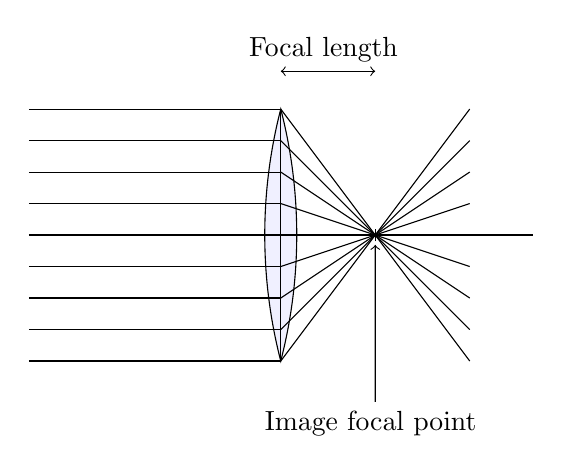
\begin{tikzpicture}[scale=0.8]
			% lens parameters
			\pgfmathsetmacro{\lensHeight}{2}
			\pgfmathsetmacro{\lensWidth}{0.75}
			\pgfmathsetmacro{\lensPos}{4}
			\pgfmathsetmacro{\lensFL}{1.5}
			\pgfmathsetmacro{\raySpacing}{0.5}

			\pgfmathsetmacro{\lensRadius}{4*\lensHeight}
			\pgfmathsetmacro{\startAngle}{asin(\lensHeight/\lensRadius)}
			\pgfmathsetmacro{\lensFm}{\lensPos-\lensFL}
			\pgfmathsetmacro{\lensFp}{\lensPos+\lensFL}

			\draw [fill=blue!30, fill opacity=0.2]  (\lensPos,\lensHeight)
			arc[start angle=180-\startAngle,delta angle=2*\startAngle,radius=\lensRadius]
			arc[start angle=-\startAngle,delta angle=2*\startAngle,radius=\lensRadius]
			-- cycle;
			\draw (\lensPos,-\lensHeight) -- (\lensPos,\lensHeight);

			% optical axis
			\draw[thick] (0,0) to (2*\lensPos,0);


			% parallel rays
			\uncover<2->{ \draw[thin]  (0,+4*\raySpacing) to (  \lensPos,+4*\raySpacing); }
			\uncover<3->{\draw[thin]  (0,+3*\raySpacing) to (  \lensPos,+3*\raySpacing); }
			\uncover<4->{\draw[thin]  (0,+2*\raySpacing) to (  \lensPos,+2*\raySpacing); }
			\uncover<5->{\draw[thin]  (0,+1*\raySpacing) to (  \lensPos,+1*\raySpacing); }
			\uncover<5->{\draw[thin]  (0,-1*\raySpacing) to (  \lensPos,-1*\raySpacing); }
			\uncover<5->{\draw[thin]  (0,-2*\raySpacing) to (  \lensPos,-2*\raySpacing); }
			\uncover<5->{\draw[thin]  (0,-3*\raySpacing) to (  \lensPos,-3*\raySpacing); }
			\uncover<5->{\draw[thin]  (0,-4*\raySpacing) to (  \lensPos,-4*\raySpacing); }

			% refracted rays
			% parameterize each line which passes through a and b as a + (b-a)t
			\pgfmathsetmacro{\lineT}{2}

			% draw a line from (\lensPos,+4*\raySpacing) to  (\lensFp, 0) and extend it by \lineT
			\uncover<2->{ \draw[thin]  (  \lensPos,+4*\raySpacing) to (\lensPos + \lineT*\lensFp - \lineT*\lensPos,4*\raySpacing-4*\lineT*\raySpacing); }

			% draw similar lines to the previous one

			\uncover<3->{ \draw[thin]  (  \lensPos,+3*\raySpacing) to (\lensPos + \lineT*\lensFp - \lineT*\lensPos, 3*\raySpacing-3*\lineT*\raySpacing); }
			\uncover<4->{ \draw[thin]  (  \lensPos,+2*\raySpacing) to (\lensPos + \lineT*\lensFp - \lineT*\lensPos, 2*\raySpacing-2*\lineT*\raySpacing); }
			\uncover<5->{ \draw[thin]  (  \lensPos,+1*\raySpacing) to (\lensPos + \lineT*\lensFp - \lineT*\lensPos, 1*\raySpacing-1*\lineT*\raySpacing); }

			\uncover<5->{ \draw[thin]  (  \lensPos,-1*\raySpacing) to (\lensPos + \lineT*\lensFp - \lineT*\lensPos,-1*\raySpacing+1*\lineT*\raySpacing); }
			\uncover<5->{ \draw[thin]  (  \lensPos,-2*\raySpacing) to (\lensPos + \lineT*\lensFp - \lineT*\lensPos,-2*\raySpacing+2*\lineT*\raySpacing); }
			\uncover<5->{ \draw[thin]  (  \lensPos,-3*\raySpacing) to (\lensPos + \lineT*\lensFp - \lineT*\lensPos,-3*\raySpacing+3*\lineT*\raySpacing); }
			\uncover<5->{ \draw[thin]  (  \lensPos,-4*\raySpacing) to (\lensPos + \lineT*\lensFp - \lineT*\lensPos,-4*\raySpacing+4*\lineT*\raySpacing); }

			% focal points
			\uncover<6->{
				\draw (\lensFp, -0.1) -- (\lensFp, 0.1);
				\node (ifpSym) at (\lensFp, 0) {};
				\node (ifpTxt) at (\lensFp, -3) {$\text{Image focal point}~\micif$};
				\path (ifpTxt) edge[->] (ifpSym);

			}
			\uncover<7->{\draw[<->] (\lensPos,1.3*\lensHeight) -- (\lensFp,1.3*\lensHeight) node[midway,above] {$\text{Focal length}~\micfl$};}

		\end{tikzpicture}
	\end{center}


\end{frame}
%%%%%%%%%%%%%%%%%%%%%%%%%%%%%%%%%%%%%%%%%%%%%%%%%%%%%%%%%%%%%%%%%%%%%%%%%%%%%%%%%%%%%%%%%%%%%%%%%%%%
%%%%%%%%%%%%%%%%%%%%%%%%%%%%%%%%%%%%%%%%%%%%%%%%%%%%%%%%%%%%%%%%%%%%%%%%%%%%%%%%%%%%%%%%%%%%%%%%%%%%
\begin{frame}{Diverging Lens}
	\begin{center}
		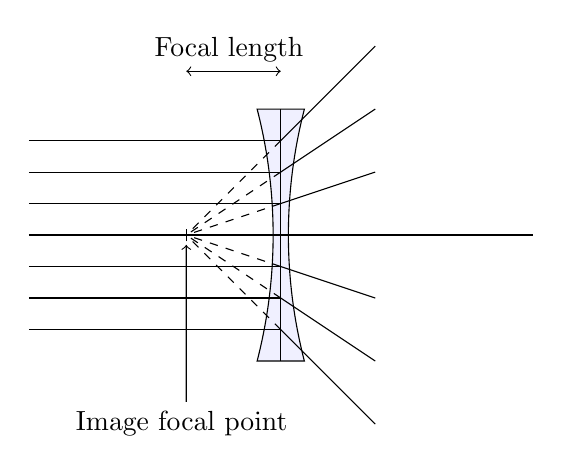
\begin{tikzpicture}[scale=0.8]
			% lens parameters
			\pgfmathsetmacro{\lensHeight}{2}
			\pgfmathsetmacro{\lensWidth}{0.75}
			\pgfmathsetmacro{\lensPos}{4}
			\pgfmathsetmacro{\lensFL}{1.5}
			\pgfmathsetmacro{\raySpacing}{0.5}

			\pgfmathsetmacro{\lensRadius}{4*\lensHeight}
			\pgfmathsetmacro{\startAngle}{asin(\lensHeight/\lensRadius)}
			\pgfmathsetmacro{\lensFm}{\lensPos-\lensFL}
			\pgfmathsetmacro{\lensFp}{\lensPos+\lensFL}

			% Concave lens
			\draw [fill=blue!30, fill opacity=0.2]  (\lensPos-0.5*\lensWidth,\lensHeight)
			arc[start angle=\startAngle,delta angle=-2*\startAngle,radius=\lensRadius]
			-- (\lensPos+0.5*\lensWidth,-\lensHeight)
			arc[start angle=180+\startAngle,delta angle=-2*\startAngle,radius=\lensRadius]
			-- cycle;
			\draw (\lensPos,-\lensHeight) -- (\lensPos,\lensHeight);
			% optical axis
			\draw[thick] (0,0) to (2*\lensPos,0);


			% parallel rays
			%\uncover<2->{ \draw[thin]  (0,+4*\raySpacing) to (  \lensPos,+4*\raySpacing); }
			\uncover<2->{\draw[thin]  (0,+3*\raySpacing) to (  \lensPos,+3*\raySpacing); }
			\uncover<3->{\draw[thin]  (0,+2*\raySpacing) to (  \lensPos,+2*\raySpacing); }
			\uncover<4->{\draw[thin]  (0,+1*\raySpacing) to (  \lensPos,+1*\raySpacing); }
			\uncover<4->{\draw[thin]  (0,-1*\raySpacing) to (  \lensPos,-1*\raySpacing); }
			\uncover<4->{\draw[thin]  (0,-2*\raySpacing) to (  \lensPos,-2*\raySpacing); }
			\uncover<4->{\draw[thin]  (0,-3*\raySpacing) to (  \lensPos,-3*\raySpacing); }
			%\uncover<5->{\draw[thin]  (0,-4*\raySpacing) to (  \lensPos,-4*\raySpacing); }

			% refracted rays
			% parameterize each line which passes through a and b as a + (b-a)t
			\pgfmathsetmacro{\lineT}{-1}

			% draw a line from (\lensPos,+4*\raySpacing) to  (\lensFm, 0) and extend it by \lineT
			%\uncover<2->{ \draw[thin]  (  \lensPos,+4*\raySpacing) to (\lensPos + \lineT*\lensFm - \lineT*\lensPos,4*\raySpacing-4*\lineT*\raySpacing); }

			% draw similar lines to the previous one

			\uncover<2->{ \draw[thin]  (  \lensPos,+3*\raySpacing) to (\lensPos + \lineT*\lensFm - \lineT*\lensPos, 3*\raySpacing-3*\lineT*\raySpacing); }
			\uncover<3->{ \draw[thin]  (  \lensPos,+2*\raySpacing) to (\lensPos + \lineT*\lensFm - \lineT*\lensPos, 2*\raySpacing-2*\lineT*\raySpacing); }
			\uncover<4->{ \draw[thin]  (  \lensPos,+1*\raySpacing) to (\lensPos + \lineT*\lensFm - \lineT*\lensPos, 1*\raySpacing-1*\lineT*\raySpacing); }

			\uncover<4->{ \draw[thin]  (  \lensPos,-1*\raySpacing) to (\lensPos + \lineT*\lensFm - \lineT*\lensPos,-1*\raySpacing+1*\lineT*\raySpacing); }
			\uncover<4->{ \draw[thin]  (  \lensPos,-2*\raySpacing) to (\lensPos + \lineT*\lensFm - \lineT*\lensPos,-2*\raySpacing+2*\lineT*\raySpacing); }
			\uncover<4->{ \draw[thin]  (  \lensPos,-3*\raySpacing) to (\lensPos + \lineT*\lensFm - \lineT*\lensPos,-3*\raySpacing+3*\lineT*\raySpacing); }
			%\uncover<5->{ \draw[thin]  (  \lensPos,-4*\raySpacing) to (\lensPos + \lineT*\lensFm - \lineT*\lensPos,-4*\raySpacing+4*\lineT*\raySpacing); }

			% draw line extensions
			\pgfmathsetmacro{\lineT}{1}
			\uncover<5->{ \draw[thin, dashed]  (  \lensPos,+3*\raySpacing) to (\lensPos + \lineT*\lensFm - \lineT*\lensPos, 3*\raySpacing-3*\lineT*\raySpacing); }
			\uncover<6->{ \draw[thin, dashed]  (  \lensPos,+2*\raySpacing) to (\lensPos + \lineT*\lensFm - \lineT*\lensPos, 2*\raySpacing-2*\lineT*\raySpacing); }
			\uncover<7->{ \draw[thin, dashed]  (  \lensPos,+1*\raySpacing) to (\lensPos + \lineT*\lensFm - \lineT*\lensPos, 1*\raySpacing-1*\lineT*\raySpacing); }

			\uncover<7->{ \draw[thin, dashed]  (  \lensPos,-1*\raySpacing) to (\lensPos + \lineT*\lensFm - \lineT*\lensPos,-1*\raySpacing+1*\lineT*\raySpacing); }
			\uncover<7->{ \draw[thin, dashed]  (  \lensPos,-2*\raySpacing) to (\lensPos + \lineT*\lensFm - \lineT*\lensPos,-2*\raySpacing+2*\lineT*\raySpacing); }
			\uncover<7->{ \draw[thin, dashed]  (  \lensPos,-3*\raySpacing) to (\lensPos + \lineT*\lensFm - \lineT*\lensPos,-3*\raySpacing+3*\lineT*\raySpacing); }
			% focal points
			\uncover<7->{
				\draw (\lensFm, -0.1) -- (\lensFm, 0.1);
				\node (ifpSym) at (\lensFm, 0) {};
				\node (ifpTxt) at (\lensFm, -3) {$\text{Image focal point}~\micif$};
				\path (ifpTxt) edge[->] (ifpSym);
			}
			\uncover<8->{\draw[<->] (\lensPos,1.3*\lensHeight) -- (\lensFm,1.3*\lensHeight) node[midway,above] {$\text{Focal length}~\micfl$};}
		\end{tikzpicture}
	\end{center}


\end{frame}
%%%%%%%%%%%%%%%%%%%%%%%%%%%%%%%%%%%%%%%%%%%%%%%%%%%%%%%%%%%%%%%%%%%%%%%%%%%%%%%%%%%%%%%%%%%%%%%%%%%%
\begin{frame}{Image Formation: Converging Lens}
	\begin{block}{Three rules:}
		\begin{columns}[T,onlytextwidth]
			\begin{column}{0.4\textwidth}
				\begin{enumerate}
					\item<3>{An incident light ray which passes through the \textbf{optical center} $\micoc$ does not suffer any refraction.}
					\item<4>{An incident light ray parallel to the optical axis is refracted passing through the \textbf{image focal point} $\micif$.}
					\item<5->{An incident light ray which passes through the \textbf{object focal point} $\micof$ is refracted parallel to the optical axis.}
				\end{enumerate}
			\end{column}
			\begin{column}{0.6\textwidth}
				\centering
				\bigskip


				\begin{tikzpicture}[scale=0.8]
					% lens parameters
					\pgfmathsetmacro{\lensHeight}{2}
					\pgfmathsetmacro{\lensWidth}{0.75}
					\pgfmathsetmacro{\lensPos}{3.5}
					\pgfmathsetmacro{\lensFL}{1.5}

					\pgfmathsetmacro{\lensRadius}{4*\lensHeight}
					\pgfmathsetmacro{\startAngle}{asin(\lensHeight/\lensRadius)}
					\pgfmathsetmacro{\lensFm}{\lensPos-\lensFL}
					\pgfmathsetmacro{\lensFp}{\lensPos+\lensFL}

					% object parameters
					\pgfmathsetmacro{\objectHeight}{1}
					\pgfmathsetmacro{\objectPos}{1}

					% calculations according to the thin lens law...
					\pgfmathsetmacro{\objectD}{\lensPos-\objectPos}
					\pgfmathsetmacro{\imageD}{\lensFL*(\lensPos-\objectPos)/(\lensPos-\objectPos-\lensFL)}
					\pgfmathsetmacro{\lensOB}{-\objectHeight*\lensFL/(\lensFm-\objectPos)}
					\pgfmathsetmacro{\imagePos}{\lensPos+\imageD}
					\pgfmathsetmacro{\imageHeight}{-\objectHeight*(\imageD)/(\objectD)}

					% coordinates for drawing
					\coordinate (objectTop) at (\objectPos,\objectHeight);
					\coordinate (objectBottom) at (\objectPos,0);
					\coordinate (imageTop) at (\imagePos,\imageHeight);
					\coordinate (imageBottom) at (\imagePos,0);
					\coordinate (lensTop) at (\lensPos,\lensHeight);
					\coordinate (lensCenter) at (\lensPos,0);
					\coordinate (lensBottom) at (\lensPos,-\lensHeight);
					\coordinate (lensOT) at (\lensPos,\objectHeight);
					\coordinate (lensOB) at (\lensPos,\lensOB);
					\coordinate (lensF1) at (\lensPos-\lensFL,0);
					\coordinate (lensF2) at (\lensPos+\lensFL,0);

					%optical axis
					\draw[thick] (0,0) to (8,0);

					% Object
					\uncover<2->{\draw[->, thick, red] (\objectPos,0) -- (objectTop) node[midway,black,left]
						{$h$};}
					% Image
					\uncover<6->{\draw[->, thick] (\imagePos,0) -- (\imagePos,\imageHeight)
						node[midway,black,right]
						{$h'$};}

					% Convex lens
					\draw [fill=blue!30, fill opacity=0.2]  (\lensPos,\lensHeight)
					arc[start angle=180-\startAngle,delta angle=2*\startAngle,radius=\lensRadius]
					arc[start angle=-\startAngle,delta angle=2*\startAngle,radius=\lensRadius]
					-- cycle;
					\draw (\lensPos,-\lensHeight) -- (\lensPos,\lensHeight);

					% focal points
					\uncover<3->{
						\node[anchor=north] at (lensCenter) {$\micoc$};}
					\uncover<4->{\draw (\lensFp, -0.1) -- (\lensFp, 0.1);
						\node[anchor=north] at (\lensFp, -0.1) {$\micif$};}
					\uncover<5->{\draw (\lensFm, -0.1) -- (\lensFm, 0.1);
						\node[anchor=north] at (\lensFm, -0.1) {$\micof$};}


					% descriptions
					\uncover<4->{\draw[<->] (\lensPos,-1.1*\lensHeight) -- (\lensFp,-1.1*\lensHeight) node[midway,below] {$\micfl$};}
					\uncover<5->{\draw[<->] (\lensPos,-1.1*\lensHeight) -- (\lensFm,-1.1*\lensHeight) node[midway,below] {$\micfl$};}

					%\draw[<->] (\lensPos,-1.2*\lensHeight) -- (\lensFm-\lensFL,-1.2*\lensHeight)
					%node[midway,below] {$2f$};
					\uncover<2->{\draw[<->] (\lensPos,1.1*\lensHeight) -- (\objectPos,1.1*\lensHeight)
						node[midway,below] {$\micod$};}
					\uncover<6->{\draw[<->] (\lensPos,1.1*\lensHeight) -- (\imagePos,1.1*\lensHeight)
						node[midway,below] {$\micid$};}

					% The rays
					\uncover<3->{\draw (objectTop) -- (lensCenter) -- (imageTop);}
					\uncover<4->{\draw (objectTop) -- (lensOT) -- (imageTop);}
					\uncover<5->{\draw (objectTop) -- (lensOB) -- (imageTop);}


				\end{tikzpicture}

			\end{column}

		\end{columns}
	\end{block}
\end{frame}
%%%%%%%%%%%%%%%%%%%%%%%%%%%%%%%%%%%%%%%%%%%%%%%%%%%%%%%%%%%%%%%%%%%%%%%%%%%%%%%%%%%%%%%%%%%%
\begin{frame}[c]{Image Formation}
	\begin{columns}[c, onlytextwidth]
		\begin{column}{0.6\textwidth}
			\begin{itemize}
				\item<1-> Two of the three rays are sufficient to form the image.
				\item<2-> An image acquired at $\micid$ is defined as an \textit{in-focus} image.
				      \begin{itemize}
					      \item<3-> At smaller or larger distances, the image is larger than a point and it is called \textit{defocused}.
				      \end{itemize}
				\item<4-> Note that $\micod > \micfl$. What does happen when:
				      \begin{itemize}
					      \item<5-> $\micod < \micfl$?
					      \item<6-> A diverging lens is used?
				      \end{itemize}
			\end{itemize}
		\end{column}\begin{column}{0.4\textwidth}
			\centering
			\bigskip


			\begin{tikzpicture}[scale=0.5]
				% lens parameters
				\pgfmathsetmacro{\lensHeight}{2}
				\pgfmathsetmacro{\lensWidth}{0.75}
				\pgfmathsetmacro{\lensPos}{3.5}
				\pgfmathsetmacro{\lensFL}{1.5}

				\pgfmathsetmacro{\lensRadius}{4*\lensHeight}
				\pgfmathsetmacro{\startAngle}{asin(\lensHeight/\lensRadius)}
				\pgfmathsetmacro{\lensFm}{\lensPos-\lensFL}
				\pgfmathsetmacro{\lensFp}{\lensPos+\lensFL}

				% object parameters
				\pgfmathsetmacro{\objectHeight}{1}
				\pgfmathsetmacro{\objectPos}{1}

				% calculations according to the thin lens law...
				\pgfmathsetmacro{\objectD}{\lensPos-\objectPos}
				\pgfmathsetmacro{\imageD}{\lensFL*(\lensPos-\objectPos)/(\lensPos-\objectPos-\lensFL)}
				\pgfmathsetmacro{\lensOB}{-\objectHeight*\lensFL/(\lensFm-\objectPos)}
				\pgfmathsetmacro{\imagePos}{\lensPos+\imageD}
				\pgfmathsetmacro{\imageHeight}{-\objectHeight*(\imageD)/(\objectD)}

				% coordinates for drawing
				\coordinate (objectTop) at (\objectPos,\objectHeight);
				\coordinate (objectBottom) at (\objectPos,0);
				\coordinate (imageTop) at (\imagePos,\imageHeight);
				\coordinate (imageBottom) at (\imagePos,0);
				\coordinate (lensTop) at (\lensPos,\lensHeight);
				\coordinate (lensCenter) at (\lensPos,0);
				\coordinate (lensBottom) at (\lensPos,-\lensHeight);
				\coordinate (lensOT) at (\lensPos,\objectHeight);
				\coordinate (lensOB) at (\lensPos,\lensOB);
				\coordinate (lensF1) at (\lensPos-\lensFL,0);
				\coordinate (lensF2) at (\lensPos+\lensFL,0);

				%optical axis
				\draw[thick] (0,0) to (8,0);

				% Object
				\uncover<1->{\draw[->, thick, red] (\objectPos,0) -- (objectTop) node[midway,black,left]
					{$h$};}
				% Image
				\uncover<1->{\draw[->, thick] (\imagePos,0) -- (\imagePos,\imageHeight)
					node[midway,black,right]
					{$h'$};}

				% Convex lens
				\draw [fill=blue!30, fill opacity=0.2]  (\lensPos,\lensHeight)
				arc[start angle=180-\startAngle,delta angle=2*\startAngle,radius=\lensRadius]
				arc[start angle=-\startAngle,delta angle=2*\startAngle,radius=\lensRadius]
				-- cycle;
				\draw (\lensPos,-\lensHeight) -- (\lensPos,\lensHeight);

				% focal points
				\uncover<1->{
					\node[anchor=north] at (lensCenter) {$\micoc$};}
				\uncover<1->{\draw (\lensFp, -0.1) -- (\lensFp, 0.1);
					\node[anchor=north] at (\lensFp, -0.1) {$\micif$};}
				\uncover<1->{\draw (\lensFm, -0.1) -- (\lensFm, 0.1);
					\node[anchor=north] at (\lensFm, -0.1) {$\micof$};}


				% descriptions
				\uncover<1->{\draw[<->] (\lensPos,-1.1*\lensHeight) -- (\lensFp,-1.1*\lensHeight) node[midway,below] {$\micfl$};}
				\uncover<1->{\draw[<->] (\lensPos,-1.1*\lensHeight) -- (\lensFm,-1.1*\lensHeight) node[midway,below] {$\micfl$};}
				%\draw[<->] (\lensPos,-1.2*\lensHeight) -- (\lensFm-\lensFL,-1.2*\lensHeight)
				%node[midway,below] {$2f$};
				\uncover<1->{\draw[<->] (\lensPos,1.1*\lensHeight) -- (\objectPos,1.1*\lensHeight)
					node[midway,below] {$\micod$};}
				\uncover<1->{\draw[<->] (\lensPos,1.1*\lensHeight) -- (\imagePos,1.1*\lensHeight)
					node[midway,below] {$\micid$};}

				% The rays
				\uncover<1->{\draw (objectTop) -- (lensCenter) -- (imageTop);}
				\uncover<1->{\draw (objectTop) -- (lensOT) -- (imageTop);}
				\uncover<1->{\draw (objectTop) -- (lensOB) -- (imageTop);}

			\end{tikzpicture}

		\end{column}




	\end{columns}
\end{frame}
%%%%%%%%%%%%%%%%%%%%%%%%%%%%%%%%%%%%%%%%%%%%%%%%%%%%%%%%%%%%%%%%%%%%%%%%%%%%%%%%%%%%%%%%%%%%%%%%%%%%
\begin{frame}{Image Formation: Converging Lens $\micod < \micfl$}
	\begin{block}{Three rules:}
		\begin{columns}[T,onlytextwidth]
			\begin{column}{0.4\textwidth}
				\begin{enumerate}
					\item<3> An incident light ray which passes through the \textbf{optical center} $\micoc$ does not suffer any refraction.
					\item<4> An incident light ray parallel to the optical axis is refracted passing through the \textbf{image focal point} $\micif$.
					\item<5-> An incident light ray which passes through the \textbf{object focal point} $\micof$ is refracted parallel to the optical axis.
				\end{enumerate}
			\end{column}
			\begin{column}{0.6\textwidth}
				\centering
				\bigskip


				\begin{tikzpicture}[scale=0.8]
					% lens parameters
					\pgfmathsetmacro{\lensHeight}{2}
					\pgfmathsetmacro{\lensWidth}{0.75}
					\pgfmathsetmacro{\lensPos}{3.5}
					\pgfmathsetmacro{\lensFL}{1.5}

					\pgfmathsetmacro{\lensRadius}{4*\lensHeight}
					\pgfmathsetmacro{\startAngle}{asin(\lensHeight/\lensRadius)}
					\pgfmathsetmacro{\lensFm}{\lensPos-\lensFL}
					\pgfmathsetmacro{\lensFp}{\lensPos+\lensFL}

					% object parameters
					\pgfmathsetmacro{\objectHeight}{1}
					\pgfmathsetmacro{\objectPos}{2.8}


					% calculations according to the thin lens law...
					\pgfmathsetmacro{\objectD}{\lensPos-\objectPos}
					\pgfmathsetmacro{\imageD}{\lensFL*(\lensPos-\objectPos)/(\lensPos-\objectPos-\lensFL)}
					\pgfmathsetmacro{\lensOB}{-\objectHeight*\lensFL/(\lensFm-\objectPos)}
					\pgfmathsetmacro{\imagePos}{\lensPos+\imageD}
					\pgfmathsetmacro{\imageHeight}{-\objectHeight*(\imageD)/(\objectD)}

					% coordinates for drawing
					\coordinate (objectTop) at (\objectPos,\objectHeight);
					\coordinate (objectBottom) at (\objectPos,0);
					\coordinate (imageTop) at (\imagePos,\imageHeight);
					\coordinate (imageBottom) at (\imagePos,0);
					\coordinate (lensTop) at (\lensPos,\lensHeight);
					\coordinate (lensCenter) at (\lensPos,0);
					\coordinate (lensBottom) at (\lensPos,-\lensHeight);
					\coordinate (lensOT) at (\lensPos,\objectHeight);
					\coordinate (lensOB) at (\lensPos,\lensOB);
					\coordinate (lensF1) at (\lensPos-\lensFL,0);
					\coordinate (lensF2) at (\lensPos+\lensFL,0);

					\pgfmathsetmacro{\tt}{3} % for line extensions
					\coordinate (ray1End) at ( {(1-\tt)*\objectPos+\tt*\lensPos},{(1-\tt)*\objectHeight+\tt*0});
					\coordinate (ray2End) at ( {(1-\tt)*\lensPos+\tt*\lensFp}   ,{(1-\tt)*\objectHeight+\tt*0});
					\coordinate (ray3End) at ( {(1-\tt)*\lensPos+\tt*\lensFp}   ,{(1-\tt)*\imageHeight+\tt*\imageHeight});
					%optical axis
					\draw[thick] (0,0) to (8,0);

					% Object
					\uncover<2->{\draw[->, thick, red] (\objectPos,0) -- (objectTop) node[midway,black,left]
						{$h$};}
					% Image
					\uncover<9->{\draw[->, thick] (\imagePos,0) -- (\imagePos,\imageHeight)
						node[midway,black,left]
						{$h'$};}

					% Convex lens
					\draw [fill=blue!30, fill opacity=0.2]  (\lensPos,\lensHeight)
					arc[start angle=180-\startAngle,delta angle=2*\startAngle,radius=\lensRadius]
					arc[start angle=-\startAngle,delta angle=2*\startAngle,radius=\lensRadius]
					-- cycle;
					\draw (\lensPos,-\lensHeight) -- (\lensPos,\lensHeight);

					% focal points
					\uncover<1->{
						\node[anchor=north] at (lensCenter) {$\micoc$};}
					\uncover<1->{\draw (\lensFp, -0.1) -- (\lensFp, 0.1);
						\node[anchor=north] at (\lensFp, -0.1) {$\micif$};}
					\uncover<1->{\draw (\lensFm, -0.1) -- (\lensFm, 0.1);
						\node[anchor=north] at (\lensFm, -0.1) {$\micof$};}


					% descriptions
					\uncover<1->{\draw[<->] (\lensPos,-1.1*\lensHeight) -- (\lensFp,-1.1*\lensHeight) node[midway,below] {$\micfl$};}
					\uncover<1->{\draw[<->] (\lensPos,-1.1*\lensHeight) -- (\lensFm,-1.1*\lensHeight) node[midway,below] {$\micfl$};}
					%\draw[<->] (\lensPos,-1.2*\lensHeight) -- (\lensFm-\lensFL,-1.2*\lensHeight)
					%node[midway,below] {$2f$};
					\uncover<2->{\draw[<->] (\lensPos,1.5*\lensHeight) -- (\objectPos,1.5*\lensHeight)
						node[midway,below] {$\micod$};}
					\uncover<9->{\draw[<->] (\lensPos,-0.4*\lensHeight) -- (\imagePos,-0.4*\lensHeight)
						node[midway,below] {$\micid$};}

					% The rays
					\uncover<3->{\draw (objectTop) -- (lensCenter) -- (ray1End);}
					\uncover<4->{\draw (objectTop) -- (lensOT) -- (ray2End);}
					\uncover<5->{\draw (objectTop) -- (lensOB) -- (ray3End);
						\draw[dashed] (lensF1) -- (objectTop);}  %you need this extension here

					% extensions of the rays
					\uncover<6->{\draw [dashed] (objectTop) -- (imageTop);}
					\uncover<7->{\draw [dashed] (lensOT) -- (imageTop);}
					\uncover<8->{\draw [dashed] (lensOB) -- (imageTop);}



				\end{tikzpicture}

			\end{column}
		\end{columns}
	\end{block}
\end{frame}
%%%%%%%%%%%%%%%%%%%%%%%%%%%%%%%%%%%%%%%%%%%%%%%%%%%%%%%%%%%%%%%%%%%%%%%%%%%%%%%%%%%%%%%%%%%
%%%%%%%%%%%%%%%%%%%%%%%%%%%%%%%%%%%%%%%%%%%%%%%%%%%%%%%%%%%%%%%%%%%%%%%%%%%%%%%%%%%%%%%%%%%%%%%%%%%%
\begin{frame}{Real and Virtual Images}
	%\begin{block}{Three rules:}
	\begin{columns}[T,onlytextwidth]
		\begin{column}{0.5\textwidth}
			\centering
			\bigskip


			\begin{tikzpicture}[scale=0.5]
				% lens parameters
				\pgfmathsetmacro{\lensHeight}{2}
				\pgfmathsetmacro{\lensWidth}{0.75}
				\pgfmathsetmacro{\lensPos}{3.5}
				\pgfmathsetmacro{\lensFL}{1.5}

				\pgfmathsetmacro{\lensRadius}{4*\lensHeight}
				\pgfmathsetmacro{\startAngle}{asin(\lensHeight/\lensRadius)}
				\pgfmathsetmacro{\lensFm}{\lensPos-\lensFL}
				\pgfmathsetmacro{\lensFp}{\lensPos+\lensFL}

				% object parameters
				\pgfmathsetmacro{\objectHeight}{1}
				\pgfmathsetmacro{\objectPos}{1}

				% calculations according to the thin lens law...
				\pgfmathsetmacro{\objectD}{\lensPos-\objectPos}
				\pgfmathsetmacro{\imageD}{\lensFL*(\lensPos-\objectPos)/(\lensPos-\objectPos-\lensFL)}
				\pgfmathsetmacro{\lensOB}{-\objectHeight*\lensFL/(\lensFm-\objectPos)}
				\pgfmathsetmacro{\imagePos}{\lensPos+\imageD}
				\pgfmathsetmacro{\imageHeight}{-\objectHeight*(\imageD)/(\objectD)}

				% coordinates for drawing
				\coordinate (objectTop) at (\objectPos,\objectHeight);
				\coordinate (objectBottom) at (\objectPos,0);
				\coordinate (imageTop) at (\imagePos,\imageHeight);
				\coordinate (imageBottom) at (\imagePos,0);
				\coordinate (lensTop) at (\lensPos,\lensHeight);
				\coordinate (lensCenter) at (\lensPos,0);
				\coordinate (lensBottom) at (\lensPos,-\lensHeight);
				\coordinate (lensOT) at (\lensPos,\objectHeight);
				\coordinate (lensOB) at (\lensPos,\lensOB);
				\coordinate (lensF1) at (\lensPos-\lensFL,0);
				\coordinate (lensF2) at (\lensPos+\lensFL,0);

				%optical axis
				\draw[thick] (0,0) to (8,0);

				% Object
				\uncover<1->{\draw[->, thick, red] (\objectPos,0) -- (objectTop) node[midway,black,left]
					{$h$};}
				% Image
				\uncover<6->{\draw[->, thick] (\imagePos,0) -- (\imagePos,\imageHeight)
					node[midway,black,right]
					{$h'$};}

				% Convex lens
				\draw [fill=blue!30, fill opacity=0.2]  (\lensPos,\lensHeight)
				arc[start angle=180-\startAngle,delta angle=2*\startAngle,radius=\lensRadius]
				arc[start angle=-\startAngle,delta angle=2*\startAngle,radius=\lensRadius]
				-- cycle;
				\draw (\lensPos,-\lensHeight) -- (\lensPos,\lensHeight);

				% focal points
				\uncover<1->{
					\node[anchor=north] at (lensCenter) {$\micoc$};}
				\uncover<1->{\draw (\lensFp, -0.1) -- (\lensFp, 0.1);
					\node[anchor=north] at (\lensFp, -0.1) {$\micif$};}
				\uncover<1->{\draw (\lensFm, -0.1) -- (\lensFm, 0.1);
					\node[anchor=north] at (\lensFm, -0.1) {$\micof$};}


				% descriptions
				\uncover<1->{\draw[<->] (\lensPos,-1.1*\lensHeight) -- (\lensFp,-1.1*\lensHeight) node[midway,below] {$\micfl$};}
				\uncover<1->{\draw[<->] (\lensPos,-1.1*\lensHeight) -- (\lensFm,-1.1*\lensHeight) node[midway,below] {$\micfl$};}
				\uncover<1->{\draw[<->] (\lensPos,1.1*\lensHeight) -- (\objectPos,1.1*\lensHeight)
					node[midway,below] {$\micod$};}
				\uncover<6->{\draw[<->] (\lensPos,1.1*\lensHeight) -- (\imagePos,1.1*\lensHeight)
					node[midway,below] {$\micid$};}

				% The rays
				\uncover<3->{\draw (objectTop) -- (lensCenter) -- (imageTop);}
				\uncover<4->{\draw (objectTop) -- (lensOT) -- (imageTop);}
				\uncover<5->{\draw (objectTop) -- (lensOB) -- (imageTop);}


			\end{tikzpicture}

			\vspace*{5mm}

			\begin{tikzpicture}[scale=0.5]
				% lens parameters
				\pgfmathsetmacro{\lensHeight}{2}
				\pgfmathsetmacro{\lensWidth}{0.75}
				\pgfmathsetmacro{\lensPos}{3.5}
				\pgfmathsetmacro{\lensFL}{1.5}

				\pgfmathsetmacro{\lensRadius}{4*\lensHeight}
				\pgfmathsetmacro{\startAngle}{asin(\lensHeight/\lensRadius)}
				\pgfmathsetmacro{\lensFm}{\lensPos-\lensFL}
				\pgfmathsetmacro{\lensFp}{\lensPos+\lensFL}

				% object parameters
				\pgfmathsetmacro{\objectHeight}{1}
				\pgfmathsetmacro{\objectPos}{2.8}


				% calculations according to the thin lens law...
				\pgfmathsetmacro{\objectD}{\lensPos-\objectPos}
				\pgfmathsetmacro{\imageD}{\lensFL*(\lensPos-\objectPos)/(\lensPos-\objectPos-\lensFL)}
				\pgfmathsetmacro{\lensOB}{-\objectHeight*\lensFL/(\lensFm-\objectPos)}
				\pgfmathsetmacro{\imagePos}{\lensPos+\imageD}
				\pgfmathsetmacro{\imageHeight}{-\objectHeight*(\imageD)/(\objectD)}

				% coordinates for drawing
				\coordinate (objectTop) at (\objectPos,\objectHeight);
				\coordinate (objectBottom) at (\objectPos,0);
				\coordinate (imageTop) at (\imagePos,\imageHeight);
				\coordinate (imageBottom) at (\imagePos,0);
				\coordinate (lensTop) at (\lensPos,\lensHeight);
				\coordinate (lensCenter) at (\lensPos,0);
				\coordinate (lensBottom) at (\lensPos,-\lensHeight);
				\coordinate (lensOT) at (\lensPos,\objectHeight);
				\coordinate (lensOB) at (\lensPos,\lensOB);
				\coordinate (lensF1) at (\lensPos-\lensFL,0);
				\coordinate (lensF2) at (\lensPos+\lensFL,0);

				\pgfmathsetmacro{\tt}{3} % for line extensions
				\coordinate (ray1End) at ( {(1-\tt)*\objectPos+\tt*\lensPos},{(1-\tt)*\objectHeight+\tt*0});
				\coordinate (ray2End) at ( {(1-\tt)*\lensPos+\tt*\lensFp}   ,{(1-\tt)*\objectHeight+\tt*0});
				\coordinate (ray3End) at ( {(1-\tt)*\lensPos+\tt*\lensFp}   ,{(1-\tt)*\imageHeight+\tt*\imageHeight});
				%optical axis
				\draw[thick] (0,0) to (8,0);

				% Object
				\uncover<1->{\draw[->, thick, red] (\objectPos,0) -- (objectTop) node[midway,black,left]
					{$h$};}
				% Image
				\uncover<6->{\draw[->, thick] (\imagePos,0) -- (\imagePos,\imageHeight)
					node[midway,black,left]
					{$h'$};}

				% Convex lens
				\draw [fill=blue!30, fill opacity=0.2]  (\lensPos,\lensHeight)
				arc[start angle=180-\startAngle,delta angle=2*\startAngle,radius=\lensRadius]
				arc[start angle=-\startAngle,delta angle=2*\startAngle,radius=\lensRadius]
				-- cycle;
				\draw (\lensPos,-\lensHeight) -- (\lensPos,\lensHeight);

				% focal points
				\uncover<1->{
					\node[anchor=north] at (lensCenter) {$\micoc$};}
				\uncover<1->{\draw (\lensFp, -0.1) -- (\lensFp, 0.1);
					\node[anchor=north] at (\lensFp, -0.1) {$\micif$};}
				\uncover<1->{\draw (\lensFm, -0.1) -- (\lensFm, 0.1);
					\node[anchor=north] at (\lensFm, -0.1) {$\micof$};}


				% descriptions
				\uncover<1->{\draw[<->] (\lensPos,-1.1*\lensHeight) -- (\lensFp,-1.1*\lensHeight) node[midway,below] {$\micfl$};}
				\uncover<1->{\draw[<->] (\lensPos,-1.1*\lensHeight) -- (\lensFm,-1.1*\lensHeight) node[midway,below] {$\micfl$};}
				%\draw[<->] (\lensPos,-1.2*\lensHeight) -- (\lensFm-\lensFL,-1.2*\lensHeight)
				%node[midway,below] {$2f$};
				\uncover<1->{\draw[<->] (\lensPos,1.2*\lensHeight) -- (\objectPos,1.2*\lensHeight)
					node[midway,below] {$\micod$};}
				\uncover<6->{\draw[<->] (\lensPos,-0.4*\lensHeight) -- (\imagePos,-0.4*\lensHeight)
					node[midway,below] {$\micid$};}

				% The rays
				\uncover<3->{\draw (objectTop) -- (lensCenter) -- (ray1End);}
				\uncover<4->{\draw (objectTop) -- (lensOT) -- (ray2End);}
				\uncover<5->{\draw (objectTop) -- (lensOB) -- (ray3End);
					\draw[dashed] (lensF1) -- (objectTop);}  %you need this extension here

				% extensions of the rays
				\uncover<5->{\draw [dashed] (objectTop) -- (imageTop);}
				\uncover<5->{\draw [dashed] (lensOT) -- (imageTop);}
				\uncover<5->{\draw [dashed] (lensOB) -- (imageTop);}



			\end{tikzpicture}
		\end{column}

		\begin{column}{0.5\textwidth}
			\centering
			\bigskip
			\begin{itemize}
				\item<7-> \textbf{Real} image: Intersection of light rays.
				      \begin{itemize}\item<8-> Can be projected on a detector.\end{itemize}
				\item<9-> Image is \textbf{inverted}.
				      \vspace*{5mm}
				\item<7-> \textbf{Virtual} image: Intersection of \underline{extensions} of light rays.
				      \begin{itemize}\item<8-> Can \underline{not} be projected on a detector.\end{itemize}
				\item<9-> Image is \textbf{upright}.
			\end{itemize}


		\end{column}
	\end{columns}
	%\end{block}
\end{frame}
%%%%%%%%%%%%%%%%%%%%%%%%%%%%%%%%%%%%%%%%%%%%%%%%%%%%%%%%%%%%%%%%%%%%%%%%%%%%%%%%%%%%%%%%%%%
%%%%%%%%%%%%%%%%%%%%%%%%%%%%%%%%%%%%%%%%%%%%%%%%%%%%%%%%%%%%%%%%%%%%%%%%%%%%%%%%%%%%%%%%%%%%%%%%%%%%
\begin{frame}{Image Formation: Diverging Lens}
	\begin{block}{Three rules:}
		\begin{columns}[T,onlytextwidth]
			\begin{column}{0.4\textwidth}
				\begin{enumerate}
					\item<3> An incident light ray which passes through the \textbf{optical center} $\micoc$ does not suffer any refraction.
					\item<4> An incident light ray parallel to the optical axis is refracted passing through the \textbf{image focal point} $\micif$.
					\item<5-> An incident light ray which passes through the \textbf{object focal point} $\micof$ is refracted parallel to the optical axis.
				\end{enumerate}
			\end{column}
			\begin{column}{0.6\textwidth}
				\centering
				\bigskip


				\begin{tikzpicture}[scale=0.8]
					% lens parameters
					\pgfmathsetmacro{\lensHeight}{2}
					\pgfmathsetmacro{\lensWidth}{0.75}
					\pgfmathsetmacro{\lensPos}{3.5}
					\pgfmathsetmacro{\lensFL}{-1.5}

					\pgfmathsetmacro{\lensRadius}{4*\lensHeight}
					\pgfmathsetmacro{\startAngle}{asin(\lensHeight/\lensRadius)}
					\pgfmathsetmacro{\lensFm}{\lensPos-\lensFL}
					\pgfmathsetmacro{\lensFp}{\lensPos+\lensFL}

					% object parameters
					\pgfmathsetmacro{\objectHeight}{1}
					\pgfmathsetmacro{\objectPos}{1}


					% calculations according to the thin lens law...
					\pgfmathsetmacro{\objectD}{\lensPos-\objectPos}
					\pgfmathsetmacro{\imageD}{\lensFL*(\lensPos-\objectPos)/(\lensPos-\objectPos-\lensFL)}
					\pgfmathsetmacro{\lensOB}{-\objectHeight*\lensFL/(\lensFm-\objectPos)}
					\pgfmathsetmacro{\imagePos}{\lensPos+\imageD}
					\pgfmathsetmacro{\imageHeight}{-\objectHeight*(\imageD)/(\objectD)}

					% coordinates for drawing
					\coordinate (objectTop) at (\objectPos,\objectHeight);
					\coordinate (objectBottom) at (\objectPos,0);
					\coordinate (imageTop) at (\imagePos,\imageHeight);
					\coordinate (imageBottom) at (\imagePos,0);
					\coordinate (lensTop) at (\lensPos,\lensHeight);
					\coordinate (lensCenter) at (\lensPos,0);
					\coordinate (lensBottom) at (\lensPos,-\lensHeight);
					\coordinate (lensOT) at (\lensPos,\objectHeight);
					\coordinate (lensOB) at (\lensPos,\lensOB);
					\coordinate (lensF1) at (\lensPos-\lensFL,0);
					\coordinate (lensF2) at (\lensPos+\lensFL,0);

					\pgfmathsetmacro{\tt}{2} % for line extensions
					\pgfmathsetmacro{\ttm}{-\tt} % for line extensions
					\coordinate (ray1End) at ( {(1-\tt)*\objectPos+\tt*\lensPos},{(1-\tt)*\objectHeight+\tt*0});
					\coordinate (ray2End) at ( {(1-\ttm)*\lensPos+\ttm*\lensFp}   ,{(1-\ttm)*\objectHeight+\ttm*0});
					\coordinate (ray3End) at ( {(1-\ttm)*\lensPos+\ttm*\lensFp}   ,{(1-\ttm)*\imageHeight+\ttm*\imageHeight});
					%optical axis
					\draw[thick] (0,0) to (8,0);

					% Object
					\uncover<2->{\draw[->, thick, red] (\objectPos,0) -- (objectTop) node[midway,black,left]
						{$h$};}
					% Image
					\uncover<7->{\draw[->, thick] (\imagePos,0) -- (\imagePos,\imageHeight)
						node[midway,black,left]
						{$h'$};}

					% Concave lens
					\draw [fill=blue!30, fill opacity=0.2]  (\lensPos-0.5*\lensWidth,\lensHeight)
					arc[start angle=\startAngle,delta angle=-2*\startAngle,radius=\lensRadius]
					-- (\lensPos+0.5*\lensWidth,-\lensHeight)
					arc[start angle=180+\startAngle,delta angle=-2*\startAngle,radius=\lensRadius]
					-- cycle;
					\draw (\lensPos,-\lensHeight) -- (\lensPos,\lensHeight);


					% focal points
					\uncover<1->{
						\node[anchor=north] at (lensCenter) {$\micoc$};}
					\uncover<1->{\draw (\lensFp, -0.1) -- (\lensFp, 0.1);
						\node[anchor=north] at (\lensFp, -0.1) {$\micif$};}
					\uncover<1->{\draw (\lensFm, -0.1) -- (\lensFm, 0.1);
						\node[anchor=north] at (\lensFm, -0.1) {$\micof$};}


					% descriptions
					\uncover<1->{\draw[<->] (\lensPos,-1.1*\lensHeight) -- (\lensFp,-1.1*\lensHeight) node[midway,below] {$\micfl$};}
					\uncover<1->{\draw[<->] (\lensPos,-1.1*\lensHeight) -- (\lensFm,-1.1*\lensHeight) node[midway,below] {$\micfl$};}
					%\draw[<->] (\lensPos,-1.2*\lensHeight) -- (\lensFm-\lensFL,-1.2*\lensHeight)
					%node[midway,below] {$2f$};
					\uncover<2->{\draw[<->] (\lensPos,1.5*\lensHeight) -- (\objectPos,1.5*\lensHeight)
						node[midway,below] {$\micod$};}
					\uncover<7->{\draw[<->] (\lensPos,-0.4*\lensHeight) -- (\imagePos,-0.4*\lensHeight)
						node[midway,below] {$\micid$};}

					% The rays
					\uncover<3->{\draw (objectTop) -- (lensCenter) -- (ray1End);}
					\uncover<4->{\draw (objectTop) -- (lensOT) -- (ray2End);\draw[dashed] (lensF2) -- (lensOT);}%you need also extension here
					\uncover<5->{\draw (objectTop) -- (lensOB) -- (ray3End);
						\draw[dashed] (lensF1) -- (lensOB);}  %you need this extension here

					% extensions of the rays
					%\uncover<6->{\draw [dashed] (objectTop) -- (imageTop);}
					%\uncover<7->{\draw [dashed] (lensOT) -- (imageTop);}
					\uncover<6->{\draw [dashed] (lensOB) -- (imageTop);}



				\end{tikzpicture}

			\end{column}
		\end{columns}
	\end{block}
\end{frame}
%%%%%%%%%%%%%%%%%%%%%%%%%%%%%%%%%%%%%%%%%%%%%%%%%%%%%%%%%%%%%%%%%%%%%%%%%%%%%%%%%%%%%%%%%%
\begin{frame}{Thin Lens Model}
	\begin{enumerate}
		\item \uncover<2->{What is the relation between $\micod$ and $\micid$?}
		\item \uncover<3->{For instance, if we know $\micfl$ and $\micod$, can we compute $\micid$ without constructing the image geometrically?}
	\end{enumerate}
\end{frame}
%%%%%%%%%%%%%%%%%%%%%%%%%%%%%%%%%%%%%%%%%%%%%%%%%%%%%%%%%%%%%%%%%%%%%%%%%%%%%%%%%%%%%%%%%%%%%%%%%%%%%%%%%%%%%%
\begin{frame}{Thin Lens Model}
	%\begin{block}{}
	\begin{columns}[T,onlytextwidth]
		\begin{column}{0.45\textwidth}
			\only<1->{
				Consider a converging lens under the condition: $\micod > \micfl$.
			}
			\only<2->{
				From the similar triangles in blue:
				\begin{equation}\label{eq:mic:tr1}
					\frac{\micih}{\micoh} = \frac{\micid}{\micod}
				\end{equation}
			}
			\only<3->{The same applies for the red triangles:
				\begin{equation}\label{eq:mic:tr2}
					\frac{\micih}{\micoh} = \frac{\micfl}{\micod-\micfl}
				\end{equation}
			}
			%Combining \eqs~\ref{eq:mic:tr1} and \eqs~\ref{eq:mic:tr2} yields the \textit{thin lens equation}:
			%\begin{equation}\label{eq:mic:tle}
			%\frac{1}{\micod} + \frac{1}{\micid} = \frac{1}{\micfl}
			%\end{equation}
		\end{column}
		\begin{column}{0.55\textwidth}
			\begin{tikzpicture}[scale=0.8]
				% lens parameters
				\pgfmathsetmacro{\lensHeight}{2}
				\pgfmathsetmacro{\lensWidth}{0.75}
				\pgfmathsetmacro{\lensPos}{3.5}
				\pgfmathsetmacro{\lensFL}{1.5}

				\pgfmathsetmacro{\lensRadius}{4*\lensHeight}
				\pgfmathsetmacro{\startAngle}{asin(\lensHeight/\lensRadius)}
				\pgfmathsetmacro{\lensFm}{\lensPos-\lensFL}
				\pgfmathsetmacro{\lensFp}{\lensPos+\lensFL}

				% object parameters
				\pgfmathsetmacro{\objectHeight}{1}
				\pgfmathsetmacro{\objectPos}{1}

				% calculations according to the thin lens law...
				\pgfmathsetmacro{\objectD}{\lensPos-\objectPos}
				\pgfmathsetmacro{\imageD}{\lensFL*(\lensPos-\objectPos)/(\lensPos-\objectPos-\lensFL)}
				\pgfmathsetmacro{\lensOB}{-\objectHeight*\lensFL/(\lensFm-\objectPos)}
				\pgfmathsetmacro{\imagePos}{\lensPos+\imageD}
				\pgfmathsetmacro{\imageHeight}{-\objectHeight*(\imageD)/(\objectD)}

				% coordinates for drawing
				\coordinate (objectTop) at (\objectPos,\objectHeight);
				\coordinate (objectBottom) at (\objectPos,0);
				\coordinate (imageTop) at (\imagePos,\imageHeight);
				\coordinate (imageBottom) at (\imagePos,0);
				\coordinate (lensTop) at (\lensPos,\lensHeight);
				\coordinate (lensCenter) at (\lensPos,0);
				\coordinate (lensBottom) at (\lensPos,-\lensHeight);
				\coordinate (lensOT) at (\lensPos,\objectHeight);
				\coordinate (lensOB) at (\lensPos,\lensOB);
				\coordinate (lensF1) at (\lensPos-\lensFL,0);
				\coordinate (lensF2) at (\lensPos+\lensFL,0);

				% Mark similar triangles
				\only<3>{
					\path[fill=red!30] (objectTop) -- (lensF1) -- (objectBottom) -- cycle;
					\path[fill=red!30] (lensF1) -- (lensCenter) -- (lensOB) -- cycle;
				}\only<2>{
					\path[fill=blue!30] (lensCenter) -- (imageTop) -- (imageBottom) -- cycle;
					\path[fill=blue!30] (objectTop) -- (lensCenter) -- (objectBottom) -- cycle;
				}

				%	 \pgfmathsetmacro{\objAngle}{atan(\objectHeight/(\lensFm-\objectPos))}
				%	 \draw[red, ultra thick] (lensF1) +(180:0.5cm) arc[start angle=180,
				%	 radius=0.5cm, delta angle=-\objAngle];
				%	 \draw[red, ultra thick] (lensF1) +(0:0.5cm) arc[start angle=0,
				%	 radius=0.5cm, delta angle=-\objAngle];

				%optical axis
				\draw[thick] (0,0) to (8,0);

				% Object
				\draw[->, thick, red] (\objectPos,0) -- (objectTop) node[midway,black,left]	{$h$};
				% Image
				\draw[->, thick] (\imagePos,0) -- (\imagePos,\imageHeight)
				node[midway,black,right]
				{$h'$};

				% The Lens
				\draw [fill=blue!30, fill opacity=0.2]  (\lensPos,\lensHeight)
				arc[start angle=180-\startAngle,delta angle=2*\startAngle,radius=\lensRadius]
				arc[start angle=-\startAngle,delta angle=2*\startAngle,radius=\lensRadius]
				-- cycle; % to get a better line end
				\draw (\lensPos,-\lensHeight) -- (\lensPos,\lensHeight);
				\draw (\lensFm, -0.1) -- (\lensFm, 0.1);
				\draw (\lensFp, -0.1) -- (\lensFp, 0.1);
				\node[anchor=north] at (\lensFm, -0.1) {$\micof$};
				\node[anchor=north] at (\lensFp, -0.1) {$\micif$};


				\draw[<->] (\lensPos,-1.1*\lensHeight) -- (\lensFm,-1.1*\lensHeight) node[midway,above] {$f$};
				\draw[<->] (\lensPos,-1.1*\lensHeight) -- (\lensFp,-1.1*\lensHeight) node[midway,above] {$f$};
				%\draw[<->] (\lensPos,-1.2*\lensHeight) -- (\lensFm-\lensFL,-1.2*\lensHeight)
				%node[midway,below] {$2f$};
				\draw[<->] (\lensPos,1.1*\lensHeight) -- (\objectPos,1.1*\lensHeight)
				node[midway,below] {$d$};
				\draw[<->] (\lensPos,1.1*\lensHeight) -- (\imagePos,1.1*\lensHeight)
				node[midway,below] {$d'$};

				% The rays
				\draw (objectTop) -- (lensCenter) -- (imageTop);
				\draw (objectTop) -- (lensOB) -- (imageTop);
				\draw (objectTop) -- (lensOT) -- (imageTop);



			\end{tikzpicture}
		\end{column}
	\end{columns}
	%\end{block}
\end{frame}
%%%%%%%%%%%%%%%%%%%%%%%%%%%%%%%%%%%%%%%%%%%%%%%%%%%%%%%%%%%%%%%%%%%%%%%%%%%%%%%%%%%%%%%%%%%%%%%%%%%%%%%%%%%%%%%%%%%%%%%%%%%%
%%%%%%%%%%%%%%%%%%%%%%%%%%%%%%%%%%%%%%%%%%%%%%%%%%%%%%%%%%%%%%%%%%%%%%%%%%%%%%%%%%%%%%%%%%%%%%%%%%%%%%%%%%%%%%%%%%%%%%%%%%%%%%%%%
\begin{frame}{Thin Lens Model}
	%\begin{block}{}
	%\setcounter{equation}{0}
	\begin{columns}[T,onlytextwidth]
		\begin{column}{0.55\textwidth}
			%\only<1>{
			%	\begin{align}%\label{eq:mic:tr1}
			%	\frac{\micih}{\micoh} &= \frac{\micid}{\micod}\\
			%	\frac{\micih}{\micoh} &= \frac{\micfl}{\micod-\micfl}
			%	\end{align}
			%	}
			\only<2->{Combining Eq.~(1) and Eq.~(2) yields: \[ \frac{\micfl}{\micod-\micfl} = \frac{\micid}{\micod}\]}
			\only<3->{ \[\micfl \micod = \micid\micod-\micid\micfl\]}
			\only<4->{ \[\micfl \micod + \micid \micfl = \micid\micod\]}
			\only<5->{Dividing by $\micfl \micod \micid$ yields:
				\begin{equation}\label{eq:mic:tle}
					\frac{1}{\micid} + \frac{1}{\micod} = \frac{1}{\micfl}
				\end{equation}}
		\end{column}
		\begin{column}{0.45\textwidth}
			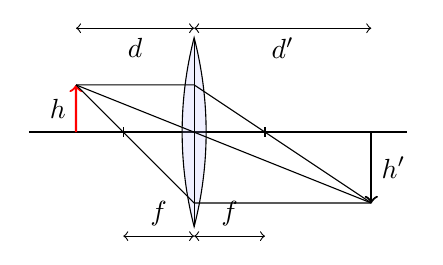
\begin{tikzpicture}[scale=0.6]
				% lens parameters
				\pgfmathsetmacro{\lensHeight}{2}
				\pgfmathsetmacro{\lensWidth}{0.75}
				\pgfmathsetmacro{\lensPos}{3.5}
				\pgfmathsetmacro{\lensFL}{1.5}

				\pgfmathsetmacro{\lensRadius}{4*\lensHeight}
				\pgfmathsetmacro{\startAngle}{asin(\lensHeight/\lensRadius)}
				\pgfmathsetmacro{\lensFm}{\lensPos-\lensFL}
				\pgfmathsetmacro{\lensFp}{\lensPos+\lensFL}

				% object parameters
				\pgfmathsetmacro{\objectHeight}{1}
				\pgfmathsetmacro{\objectPos}{1}

				% calculations according to the thin lens law...
				\pgfmathsetmacro{\objectD}{\lensPos-\objectPos}
				\pgfmathsetmacro{\imageD}{\lensFL*(\lensPos-\objectPos)/(\lensPos-\objectPos-\lensFL)}
				\pgfmathsetmacro{\lensOB}{-\objectHeight*\lensFL/(\lensFm-\objectPos)}
				\pgfmathsetmacro{\imagePos}{\lensPos+\imageD}
				\pgfmathsetmacro{\imageHeight}{-\objectHeight*(\imageD)/(\objectD)}

				% coordinates for drawing
				\coordinate (objectTop) at (\objectPos,\objectHeight);
				\coordinate (objectBottom) at (\objectPos,0);
				\coordinate (imageTop) at (\imagePos,\imageHeight);
				\coordinate (imageBottom) at (\imagePos,0);
				\coordinate (lensTop) at (\lensPos,\lensHeight);
				\coordinate (lensCenter) at (\lensPos,0);
				\coordinate (lensBottom) at (\lensPos,-\lensHeight);
				\coordinate (lensOT) at (\lensPos,\objectHeight);
				\coordinate (lensOB) at (\lensPos,\lensOB);
				\coordinate (lensF1) at (\lensPos-\lensFL,0);
				\coordinate (lensF2) at (\lensPos+\lensFL,0);


				%	 \pgfmathsetmacro{\objAngle}{atan(\objectHeight/(\lensFm-\objectPos))}
				%	 \draw[red, ultra thick] (lensF1) +(180:0.5cm) arc[start angle=180,
				%	 radius=0.5cm, delta angle=-\objAngle];
				%	 \draw[red, ultra thick] (lensF1) +(0:0.5cm) arc[start angle=0,
				%	 radius=0.5cm, delta angle=-\objAngle];

				%optical axis
				\draw[thick] (0,0) to (8,0);

				% Object
				\draw[->, thick, red] (\objectPos,0) -- (objectTop) node[midway,black,left]	{$h$};
				% Image
				\draw[->, thick] (\imagePos,0) -- (\imagePos,\imageHeight)
				node[midway,black,right]
				{$h'$};

				% The Lens
				\draw [fill=blue!30, fill opacity=0.2]  (\lensPos,\lensHeight)
				arc[start angle=180-\startAngle,delta angle=2*\startAngle,radius=\lensRadius]
				arc[start angle=-\startAngle,delta angle=2*\startAngle,radius=\lensRadius]
				-- cycle; % to get a better line end
				\draw (\lensPos,-\lensHeight) -- (\lensPos,\lensHeight);
				\draw (\lensFm, -0.1) -- (\lensFm, 0.1);
				\draw (\lensFp, -0.1) -- (\lensFp, 0.1);
				\node[anchor=north] at (\lensFm, -0.1) {$\micof$};
				\node[anchor=north] at (\lensFp, -0.1) {$\micif$};


				\draw[<->] (\lensPos,-1.1*\lensHeight) -- (\lensFm,-1.1*\lensHeight) node[midway,above] {$f$};
				\draw[<->] (\lensPos,-1.1*\lensHeight) -- (\lensFp,-1.1*\lensHeight) node[midway,above] {$f$};
				%\draw[<->] (\lensPos,-1.2*\lensHeight) -- (\lensFm-\lensFL,-1.2*\lensHeight)
				%node[midway,below] {$2f$};
				\draw[<->] (\lensPos,1.1*\lensHeight) -- (\objectPos,1.1*\lensHeight)
				node[midway,below] {$d$};
				\draw[<->] (\lensPos,1.1*\lensHeight) -- (\imagePos,1.1*\lensHeight)
				node[midway,below] {$d'$};

				% The rays
				\draw (objectTop) -- (lensCenter) -- (imageTop);
				\draw (objectTop) -- (lensOB) -- (imageTop);
				\draw (objectTop) -- (lensOT) -- (imageTop);

			\end{tikzpicture}
		\end{column}
	\end{columns}
	%\end{block}
\end{frame}
%%%%%%%%%%%%%%%%%%%%%%%%%%%%%%%%%%%%%%%%%%%%%%%%%%%%%%%%%%%%%%%%%%%%%%%%%%%%%%%%%%%%%%%%%%%%%%%%%%%%%%%%%%%%%%%%%%%%%%%%%%%%%%%%%
\begin{frame}[c]{Thin Lens Model: Generalization}
	\begin{itemize}
		\setlength\itemsep{.4cm}
		\item<1-> The thin lens equation was derived here for real images in a converging lens.
		\item<2-> Nevertheless, it can also be applied for virtual images and~/~or diverging lenses under the following sign conventions:
		      \begin{itemize}
			      \item<3-> $\micid < 0$ when the image is at the object side of the lens.
			      \item<4-> $\micfl < 0$ for diverging lenses.
		      \end{itemize}
		\item<5-> With a third sign convention stating that $\micih < 0$ for inverted images, Eq.~(1) and Eq.~(2) can be generalized to:
		      \begin{equation}\label{eq:mic:mag}
			      {\miclm} = \frac{\micih}{\micoh} = - \frac{\micfl}{\micod-\micfl} = - \frac{\micid}{\micod},
		      \end{equation}
		      where $\miclm$ is the maginification.
	\end{itemize}
\end{frame}
%%%%%%%%%%%%%%%%%%%%%%%%%%%%%%%%%%%%%%%%%%%%%%%%%%%%%%%%%%%%%%%%%%%%%%%%%%%%%%%%%%%%%%%%%%%%%%%%%%%%%%%%%%%%%%
%%%%%%%%%%%%%%%%%%%%%%%%%%%%%%%%%%%%%%%%%%%%%%%%%%%%%%%%%%%%%%%%%%%%%%%%%%%%%%%%%%%%%%%%%%%%%%%%%%%%%%%%%%%%%%%%%%%%%%%%%%%%%%%%%
\begin{frame}[c]{Magnification}

	\uncover<1-> {\[{\miclm} = \frac{\micih}{\micoh} = - \frac{\micfl}{\micod-\micfl} = - \frac{\micid}{\micod}\]}
	\vspace{0.4cm}
	\uncover<2-> {Conclusions:}
	\begin{itemize}
		\setlength\itemsep{0.4cm}
		\item<3-> The image of an object in a \textbf{converging} lens is:
		      \begin{itemize}
			      \item<4-> Magnified ($\left|\miclm\right| > 1$) when $\micod < 2 \micfl$.
			      \item<5-> Has the same size of the object when $\micod = 2 \micfl$.
			      \item<6-> Demagnified ($\left|\miclm\right| < 1$) when $\micod > 2 \micfl$.
		      \end{itemize}
		\item<7-> The image of an object in a \textbf{diverging} lens ($\micfl < 0$) is demagnified.
	\end{itemize}

\end{frame}
%%%%%%%%%%%%%%%%%%%%%%%%%%%%%%%%%%%%%%%%%%%%%%%%%%%%%%%%%%%%%%%%%%%%%%%%%%%%%%%%%%%%%%%%%%%%%%%%%%%%%%%%%%%%%%
%\begin{frame}{Outline}
%\begin{itemize}
%\item Thin Lens Model
%\item \textbf<2->{Compound Microscope}
%\item Bright Field Microscopy
%\item Fluorescence Microscopy
%\item Phase Contrast Microscopy
%\item Limitation of Light Microscopy
%\item Beyond Light Microscopy
%\item Future Trends
%\end{itemize}
%\end{frame}

\subsection{Compound Microscope}
%%%%%%%%%%%%%%%%%%%%%%%%%%%%%%%%%%%%%%%%%%%%%%%%%%%%%%%%%%%%%%%%%%%%%%%%%%%%%%%%%%%%%%%%%%%%%%%%%%%%%%%%%%%%%%
%%%%%%%%%%%%%%%%%%%%%%%%%%%%%%%%%%%%%%%%%%%%%%%%%%%%%%%%%%%%%%%%%%%%%%%%%%%%%%%%%%%%%%%%%%%%%%%%%%%%%%%%%%%%%%%%%%%%%%%%%%%%%%%%%
\begin{frame}{Compound Microscope}
	\begin{itemize}
		\item<1-> Combine two lenses:
		      \begin{itemize}
			      \item<2-> \textbf{Objective}: close to the specimen.
			      \item<3-> \textbf{Eyepiece}: Through which a user of the microscope can observe the specimen.
		      \end{itemize}
	\end{itemize}


	\begin{tikzpicture}[x=25, y=20]
		% object parameters
		\pgfmathsetmacro{\objectHeight}{0.7}
		\pgfmathsetmacro{\objectPos}{2.25}

		% objective lens parameters
		\pgfmathsetmacro{\objPos}{3.5}
		\pgfmathsetmacro{\objFL}{0.75}
		\pgfmathsetmacro{\objHeight}{1.25}

		\pgfmathsetmacro{\objRadius}{3*\objHeight}
		\pgfmathsetmacro{\objstartAngle}{asin(\objHeight/\objRadius)}
		\pgfmathsetmacro{\objFm}{\objPos-\objFL}
		\pgfmathsetmacro{\objFp}{\objPos+\objFL}

		% eyepiece/okkular lens parameters
		\pgfmathsetmacro{\okkPos}{7.5}
		\pgfmathsetmacro{\okkFL}{3}
		\pgfmathsetmacro{\okkHeight}{3}

		\pgfmathsetmacro{\okkRadius}{3*\okkHeight}
		\pgfmathsetmacro{\okkstartAngle}{asin(\okkHeight/\okkRadius)}
		\pgfmathsetmacro{\okkFm}{\okkPos-\okkFL}
		\pgfmathsetmacro{\okkFp}{\okkPos+\okkFL}

		% calculations after the thin lens law...
		\pgfmathsetmacro{\objectD}{\objPos-\objectPos}
		\pgfmathsetmacro{\imageD}{\objFL*(\objPos-\objectPos)/(\objPos-\objectPos-\objFL)}
		\pgfmathsetmacro{\objOB}{-\objectHeight*\objFL/(\objFm-\objectPos)}

		% calculation of the first image
		\pgfmathsetmacro{\imagePos}{\objPos+\imageD}
		\pgfmathsetmacro{\imageHeight}{-\objectHeight*(\imageD)/(\objectD)}

		% calculation of the final, imaginary image
		\pgfmathsetmacro{\imageDOkk}{\okkPos-\imagePos}
		\pgfmathsetmacro{\fImageD}{\okkFL*(\imageDOkk)/(\imageDOkk-\okkFL)}
		\pgfmathsetmacro{\fImagePos}{\okkPos+\fImageD}
		\pgfmathsetmacro{\fImageHeight}{-\imageHeight*(\fImageD)/(\imageDOkk)}

		% coordinates for drawing
		\coordinate (objectTop) at (\objectPos,\objectHeight);
		\coordinate (imageTop) at (\imagePos,\imageHeight);
		\coordinate (fImageTop) at (\fImagePos,\fImageHeight);

		\coordinate (objTop) at (\objPos,\objHeight);
		\coordinate (objCenter) at (\objPos,0);
		\coordinate (objBottom) at (\objPos,-\objHeight);
		\coordinate (objOT) at (\objPos,\objectHeight);
		\coordinate (objOB) at (\objPos,\objOB);
		\coordinate (objF1) at (\objPos-\objFL,0);
		\coordinate (objF2) at (\objPos+\objFL,0);

		\coordinate (okkTop) at(\okkPos,\okkHeight);
		\coordinate (okkCenter) at (\okkPos,0);
		\coordinate (okkBottom) at(\okkPos,-\okkHeight);
		\coordinate (okkOT) at (\okkPos,\imageHeight);
		\coordinate (okkF1) at (\okkPos-\okkFL,0);
		\coordinate (okkF2) at (\okkPos+\okkFL,0);

		% optical axis
		\uncover<2->{\draw[thick] (0,0) to (11,0);}

		% Object
		%\uncover<2->{
		%		\draw[->, thick, red] (\objectPos,0) -- (objectTop) node[midway,black,left]
		%		{$\scriptstyle h$};
		%		}
		% Image
		%		\uncover<4->{\draw[->, thick] (\imagePos,0) -- (\imagePos,\imageHeight)
		%		node[midway,black,right]
		%		{$\scriptstyle h'$};}
		% Final Image
		%		\uncover<7->{\draw[->, thick] (\fImagePos,0) -- (\fImagePos,\fImageHeight) node[midway,black,left]
		%		{$\scriptstyle h''$};}

		% The Lens -- Objektiv
		\uncover<2->{\draw [fill=blue!30, fill opacity=0.2]  (\objPos,\objHeight)
			arc[start angle=180-\objstartAngle,delta angle=2*\objstartAngle,radius=\objRadius]
			arc[start angle=-\objstartAngle,delta angle=2*\objstartAngle,radius=\objRadius]
			-- cycle;
			\draw (\objPos,-\objHeight) -- (\objPos,\objHeight);
			% focal points
			\draw (\objFm, -0.1) -- (\objFm, 0.1);
			\draw (\objFp, -0.1) -- (\objFp, 0.1);
			\node[anchor=north] at (\objFm, -0.1) {$\scriptstyle \miccoof$};}

		% The Lens -- Okkular
		\uncover<3->{
			\draw [fill=blue!30, fill opacity=0.2]  (\okkPos,\okkHeight)
			arc[start angle=180-\okkstartAngle,delta angle=2*\okkstartAngle,radius=\okkRadius]
			arc[start angle=-\okkstartAngle,delta angle=2*\okkstartAngle,radius=\okkRadius]
			-- cycle;
			\draw (\okkPos,-\okkHeight) -- (\okkPos,\okkHeight);
			% focal points
			\draw (\okkFm, -0.1) -- (\okkFm, 0.1);
			\draw (\okkFp, -0.1) -- (\okkFp, 0.1);
			\node[anchor=south] at (\okkFm, 0.1) {$\scriptstyle \micceof$};
			\node[anchor=north] at (\okkFp, -0.1) {$\scriptstyle \micceif$};}

		% descriptions
		\uncover<3->{\draw[<->] (\okkPos,1.3*\objHeight) -- (\okkFm,1.3*\objHeight)
			node[midway,above] {$\scriptstyle \miccefl$};}
		\uncover<2->{\draw[<->] (\objPos,1.3*\objHeight) -- (\objFm,1.3*\objHeight)
			node[midway,above] {$\scriptstyle \miccofl$};}
		%\uncover<2->{\draw[<->] (\objPos,1.1*\objHeight) -- (\objectPos,1.1*\objHeight)
		%node[left,below] {$\scriptstyle \miccofl<\miccood < 2\miccofl$};}
		%\uncover<4->{\draw[<->] (\objPos,1.1*\objHeight) -- (\imagePos,1.1*\objHeight)
		%node[midway,below] {$\scriptstyle \miccoid$};}
		%\uncover<5->{\draw[<->] (\imagePos,1.1*\objHeight) -- (\okkPos,1.1*\objHeight)
		%node[midway,below] {$\scriptstyle \micceod < \miccefl$};}
		%\uncover<7->{\draw[<->] (\okkPos,1.05*\fImageHeight) -- (\fImagePos,1.05*\fImageHeight)
		%node[midway,below] {$\scriptstyle \micceid$};}%
		%\draw[<->] (\objPos,1.05*\okkHeight) -- (\okkPos,1.05*\okkHeight)
		%node[midway,below] {$\scriptstyle t$};
		% The rays
		% objective rays
		%\uncover<3->{
		%\draw (objectTop) -- (objCenter) -- (imageTop);
		%\draw (objectTop) -- (objOT) -- (imageTop);
		%}
		% okkular rays
		%\uncover<6->{
		%\draw[shorten >=-20] (imageTop) -- (okkOT) -- (okkF2);
		%\draw[dashed] (okkOT) -- (fImageTop);
		%\draw[shorten >=-95] (imageTop) -- (okkCenter);
		%\draw[dashed] (imageTop) -- (fImageTop);}


		\uncover<2->{\node[fill=white,anchor=north, inner sep=0pt] at (\objFp, -0.25) {$\scriptstyle \miccoif$};}

		% labels of the two lenses
		\uncover<2->{\node[anchor=north, inner sep=1pt] at (objBottom) {\small Objective};}
		\uncover<3->{\node[anchor=north, inner sep=1pt] at (okkBottom) {\small Eyepiece};}
	\end{tikzpicture}
	%\end{center}


\end{frame}
%%%%%%%%%%%%%%%%%%%%%%%%%%%%%%%%%%%%%%%%%%%%%%%%%%%%%%%%%%%%%%%%%%%%%%%%%%%%%%%%%%%%%%%%%%%%%%%%%%%%%%%%%%%%%%
\begin{frame}{Compound Microscope}
	\begin{center}
		\begin{tikzpicture}[x=25, y=20]
			% object parameters
			\pgfmathsetmacro{\objectHeight}{0.7}
			\pgfmathsetmacro{\objectPos}{2.25}

			% objective lens parameters
			\pgfmathsetmacro{\objPos}{3.5}
			\pgfmathsetmacro{\objFL}{0.75}
			\pgfmathsetmacro{\objHeight}{1.25}

			\pgfmathsetmacro{\objRadius}{3*\objHeight}
			\pgfmathsetmacro{\objstartAngle}{asin(\objHeight/\objRadius)}
			\pgfmathsetmacro{\objFm}{\objPos-\objFL}
			\pgfmathsetmacro{\objFp}{\objPos+\objFL}

			% eyepiece/okkular lens parameters
			\pgfmathsetmacro{\okkPos}{7.5}
			\pgfmathsetmacro{\okkFL}{3}
			\pgfmathsetmacro{\okkHeight}{3}

			\pgfmathsetmacro{\okkRadius}{3*\okkHeight}
			\pgfmathsetmacro{\okkstartAngle}{asin(\okkHeight/\okkRadius)}
			\pgfmathsetmacro{\okkFm}{\okkPos-\okkFL}
			\pgfmathsetmacro{\okkFp}{\okkPos+\okkFL}

			% calculations after the thin lens law...
			\pgfmathsetmacro{\objectD}{\objPos-\objectPos}
			\pgfmathsetmacro{\imageD}{\objFL*(\objPos-\objectPos)/(\objPos-\objectPos-\objFL)}
			\pgfmathsetmacro{\objOB}{-\objectHeight*\objFL/(\objFm-\objectPos)}

			% calculation of the first image
			\pgfmathsetmacro{\imagePos}{\objPos+\imageD}
			\pgfmathsetmacro{\imageHeight}{-\objectHeight*(\imageD)/(\objectD)}

			% calculation of the final, imaginary image
			\pgfmathsetmacro{\imageDOkk}{\okkPos-\imagePos}
			\pgfmathsetmacro{\fImageD}{\okkFL*(\imageDOkk)/(\imageDOkk-\okkFL)}
			\pgfmathsetmacro{\fImagePos}{\okkPos+\fImageD}
			\pgfmathsetmacro{\fImageHeight}{-\imageHeight*(\fImageD)/(\imageDOkk)}

			% coordinates for drawing
			\coordinate (objectTop) at (\objectPos,\objectHeight);
			\coordinate (imageTop) at (\imagePos,\imageHeight);
			\coordinate (fImageTop) at (\fImagePos,\fImageHeight);

			\coordinate (objTop) at (\objPos,\objHeight);
			\coordinate (objCenter) at (\objPos,0);
			\coordinate (objBottom) at (\objPos,-\objHeight);
			\coordinate (objOT) at (\objPos,\objectHeight);
			\coordinate (objOB) at (\objPos,\objOB);
			\coordinate (objF1) at (\objPos-\objFL,0);
			\coordinate (objF2) at (\objPos+\objFL,0);

			\coordinate (okkTop) at(\okkPos,\okkHeight);
			\coordinate (okkCenter) at (\okkPos,0);
			\coordinate (okkBottom) at(\okkPos,-\okkHeight);
			\coordinate (okkOT) at (\okkPos,\imageHeight);
			\coordinate (okkF1) at (\okkPos-\okkFL,0);
			\coordinate (okkF2) at (\okkPos+\okkFL,0);

			% optical axis
			\draw[thick] (0,0) to (11,0);

			% Object
			\uncover<2->{
				\draw[->, thick, red] (\objectPos,0) -- (objectTop) node[midway,black,left]
				{$\scriptstyle h$};
			}
			% Image
			\uncover<4->{\draw[->, thick] (\imagePos,0) -- (\imagePos,\imageHeight)
				node[midway,black,right]
				{$\scriptstyle h'$};}
			% Final Image
			\uncover<7->{\draw[->, thick] (\fImagePos,0) -- (\fImagePos,\fImageHeight) node[midway,black,left]
				{$\scriptstyle h''$};}

			% The Lens -- Objektiv
			\draw [fill=blue!30, fill opacity=0.2]  (\objPos,\objHeight)
			arc[start angle=180-\objstartAngle,delta angle=2*\objstartAngle,radius=\objRadius]
			arc[start angle=-\objstartAngle,delta angle=2*\objstartAngle,radius=\objRadius]
			-- cycle;
			\draw (\objPos,-\objHeight) -- (\objPos,\objHeight);
			% focal points
			\draw (\objFm, -0.1) -- (\objFm, 0.1);
			\draw (\objFp, -0.1) -- (\objFp, 0.1);
			\node[anchor=north] at (\objFm, -0.1) {$\scriptstyle \miccoof$};

			% The Lens -- Okkular
			\draw [fill=blue!30, fill opacity=0.2]  (\okkPos,\okkHeight)
			arc[start angle=180-\okkstartAngle,delta angle=2*\okkstartAngle,radius=\okkRadius]
			arc[start angle=-\okkstartAngle,delta angle=2*\okkstartAngle,radius=\okkRadius]
			-- cycle;
			\draw (\okkPos,-\okkHeight) -- (\okkPos,\okkHeight);
			% focal points
			\draw (\okkFm, -0.1) -- (\okkFm, 0.1);
			\draw (\okkFp, -0.1) -- (\okkFp, 0.1);
			\node[anchor=south] at (\okkFm, 0.1) {$\scriptstyle \micceof$};
			\node[anchor=north] at (\okkFp, -0.1) {$\scriptstyle \micceif$};

			% descriptions
			\draw[<->] (\okkPos,1.3*\objHeight) -- (\okkFm,1.3*\objHeight)
			node[midway,above] {$\scriptstyle \miccefl$};
			\draw[<->] (\objPos,1.3*\objHeight) -- (\objFm,1.3*\objHeight)
			node[midway,above] {$\scriptstyle \miccofl$};
			\uncover<2->{\draw[<->] (\objPos,1.1*\objHeight) -- (\objectPos,1.1*\objHeight)
				node[left,below] {$\scriptstyle \miccofl<\miccood < 2\miccofl$};}
			\uncover<4->{\draw[<->] (\objPos,1.1*\objHeight) -- (\imagePos,1.1*\objHeight)
				node[midway,below] {$\scriptstyle \miccoid$};}
			\uncover<5->{\draw[<->] (\imagePos,1.1*\objHeight) -- (\okkPos,1.1*\objHeight)
				node[midway,below] {$\scriptstyle \micceod < \miccefl$};}
			\uncover<7->{\draw[<->] (\okkPos,1.05*\fImageHeight) -- (\fImagePos,1.05*\fImageHeight)
				node[midway,below] {$\scriptstyle \micceid$};}%
			%\draw[<->] (\objPos,1.05*\okkHeight) -- (\okkPos,1.05*\okkHeight)
			%node[midway,below] {$\scriptstyle t$};
			% The rays
			% objective rays
			\uncover<3->{
				\draw (objectTop) -- (objCenter) -- (imageTop);
				\draw (objectTop) -- (objOT) -- (imageTop);
			}
			% okkular rays
			\uncover<6->{
				\draw[shorten >=-20] (imageTop) -- (okkOT) -- (okkF2);
				\draw[dashed] (okkOT) -- (fImageTop);
				\draw[shorten >=-95] (imageTop) -- (okkCenter);
				\draw[dashed] (imageTop) -- (fImageTop);}

			% focal point of objective, draw here, to draw on top of rays
			\node[fill=white,anchor=north, inner sep=0pt] at (\objFp, -0.25) {$\scriptstyle \miccoif$};

			% labels of the two lenses
			\node[anchor=north, inner sep=1pt] at (objBottom) {\small Objective};
			\node[anchor=north, inner sep=1pt] at (okkBottom) {\small Eyepiece};
		\end{tikzpicture}
	\end{center}
	\vspace{-\bigskipamount}
	\begin{itemize}
		\item<4-> Objective image: \textbf{real} ($\miccood > \miccofl$) and \textbf{magnified} ($\miccood < 2\miccofl$).
		\item<7-> Eyepiece image: \textbf{virtual} ($\micceod < \miccefl$) and \textbf{magnified} ($\micceod < 2\miccefl$).
	\end{itemize}
\end{frame}
%%%%%%%%%%%%%%%%%%%%%%%%%%%%%%%%%%%%%%%%%%%%%%%%%%%%%%%%%%%%%%%%%%%%%%%%%%%%%%%%%%%%%%%%%%%%%%%%%%%%
%%%%%%%%%%%%%%%%%%%%%%%%%%%%%%%%%%%%%%%%%%%%%%%%%%%%%%%%%%%%%%%%%%%%%%%%%%%%%%%%%%%%%%%%%%%%%%%%%%%%%%%%%%%%%%%%%%%%%%%%%%%%%%%%%
\begin{frame}{Compound Microscope}
	\begin{itemize}
		\setlength\itemsep{0.4cm}
		\item<1-> Total magnification is the product of the two magnifications $\miclm_{\text{Total}} = \miccolm \miccelm$.
		\item<2-> The principle of compound microscope models only the magnification mechanism.
		\item<3-> How to illuminate the sample?
		\item<4-> Which kind of information is carried by light rays?
		\item<5-> Depending on how we address these questions, light microscopes can be further classified into:
		      \begin{itemize}
			      \item<2-> bright field.
			      \item<5-> phase contrast.
			      \item<6-> fluorescence-based.
			      \item<7-> \dots.
		      \end{itemize}
	\end{itemize}
\end{frame}
%%%%%%%%%%%%%%%%%%%%%%%%%%%%%%%%%%%%%%%%%%%%%%%%%%%%%%%%%%%%%%%%%%%%%%%%%%%%%%%%%%%%%%%%%%%%%%%%%%%%
%%%%%%%%%%%%%%%%%%%%%%%%%%%%%%%%%%%%%%%%%%%%%%%%%%%%%%%%%%%%%%%%%%%%%%%%%%%%%%%%%%%%%%%%%%%%%%%%%%%%%%%%%%%%%%%%%%%%%%%%%%%%%%%%%
\begin{frame}{Numerical Aperture}
	\begin{columns}[c,onlytextwidth]
		\begin{column}{0.6\textwidth}
			\begin{itemize}
				\item<1-> In modern microscopes, the objective lens is characterized by its magnification and numerical aperture.
				\item<2-> The numerical aperture quantifies the capability of a lens to gather light:
				      \begin{equation*}\label{eq:mic:na}
					      \micna = \micri~ \sin\micla
				      \end{equation*}
				      \vspace{-3mm}
				      \begin{itemize}
					      \item<3-> $\micri$ is the refractive index of the medium between the objective lens and the specimen.
					            \begin{itemize}
						            \item<4-> Eg. $\micri_{\text{air}} \approx 1$, $\micri_{\text{water}} \approx 1.33$, and $\micri_{\text{oil}} \approx 1.51$.
					            \end{itemize}
					      \item<5-> $\micla$ is the half angle of the maximum light cone which the lens can collect.
				      \end{itemize}
			\end{itemize}
		\end{column}\begin{column}{0.3\textwidth}
			\centering{}
			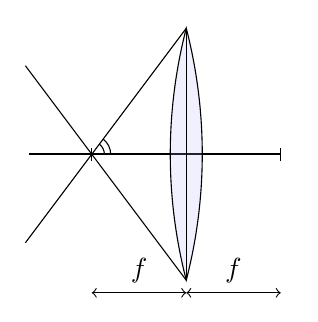
\begin{tikzpicture}[scale = 0.8]
				\pgfmathsetmacro{\lensHeight}{2}
				\pgfmathsetmacro{\lensWidth}{0.75}
				\pgfmathsetmacro{\lensPos}{3.5}
				\pgfmathsetmacro{\lensFL}{1.5}

				\pgfmathsetmacro{\lensRadius}{4*\lensHeight}
				\pgfmathsetmacro{\startAngle}{asin(\lensHeight/\lensRadius)}
				\pgfmathsetmacro{\lensFm}{\lensPos-\lensFL}
				\pgfmathsetmacro{\lensFp}{\lensPos+\lensFL}

				% object parameters
				\pgfmathsetmacro{\objectHeight}{1}
				\pgfmathsetmacro{\objectPos}{1}

				% calculations according to the thin lens law...
				\pgfmathsetmacro{\objectD}{\lensPos-\objectPos}
				\pgfmathsetmacro{\imageD}{\lensFL*(\lensPos-\objectPos)/(\lensPos-\objectPos-\lensFL)}
				\pgfmathsetmacro{\lensOB}{-\objectHeight*\lensFL/(\lensFm-\objectPos)}
				\pgfmathsetmacro{\imagePos}{\lensPos+\imageD}
				\pgfmathsetmacro{\imageHeight}{-\objectHeight*(\imageD)/(\objectD)}

				% coordinates for drawing
				\coordinate (objectTop) at (\objectPos,\objectHeight);
				\coordinate (objectBottom) at (\objectPos,0);
				\coordinate (imageTop) at (\imagePos,\imageHeight);
				\coordinate (imageBottom) at (\imagePos,0);
				\coordinate (lensTop) at (\lensPos,\lensHeight);
				\coordinate (lensCenter) at (\lensPos,0);
				\coordinate (lensBottom) at (\lensPos,-\lensHeight);
				\coordinate (lensOT) at (\lensPos,\objectHeight);
				\coordinate (lensOB) at (\lensPos,\lensOB);
				\coordinate (lensF1) at (\lensPos-\lensFL,0);
				\coordinate (lensF2) at (\lensPos+\lensFL,0);


				%	 \pgfmathsetmacro{\objAngle}{atan(\objectHeight/(\lensFm-\objectPos))}
				%	 \draw[red, ultra thick] (lensF1) +(180:0.5cm) arc[start angle=180,
				%	 radius=0.5cm, delta angle=-\objAngle];
				%	 \draw[red, ultra thick] (lensF1) +(0:0.5cm) arc[start angle=0,
				%	 radius=0.5cm, delta angle=-\objAngle];

				%optical axis
				\draw[thick] (1,0) to (5,0);

				% The Lens
				\draw [fill=blue!30, fill opacity=0.2]  (\lensPos,\lensHeight)
				arc[start angle=180-\startAngle,delta angle=2*\startAngle,radius=\lensRadius]
				arc[start angle=-\startAngle,delta angle=2*\startAngle,radius=\lensRadius]
				-- cycle; % to get a better line end
				\draw (\lensPos,-\lensHeight) -- (\lensPos,\lensHeight);
				\draw (\lensFm, -0.1) -- (\lensFm, 0.1);
				\draw (\lensFp, -0.1) -- (\lensFp, 0.1);
				\node[anchor=north] at (\lensFm, -0.1) {$\micof$};
				\node[anchor=north] at (\lensFp, -0.1) {$\micif$};


				\draw[<->] (\lensPos,-1.1*\lensHeight) -- (\lensFm,-1.1*\lensHeight) node[midway,above] {$f$};
				\draw[<->] (\lensPos,-1.1*\lensHeight) -- (\lensFp,-1.1*\lensHeight) node[midway,above] {$f$};

				% The rays
				\draw[shorten >=-40] (lensTop) -- (lensF1);
				\draw[shorten >=-40] (lensBottom) -- (lensF1);

				% angle
				\uncover<5->{
					\pgfmathsetmacro{\arcAngle}{atan(\lensHeight/\lensFL)}
					\draw (\lensFm+0.2,0) arc (0:\arcAngle:0.2);
					\draw (\lensFm+0.3,0) arc (0:\arcAngle:0.3);
					\node[anchor=north, inner sep=1pt] at (\lensFm+0.5,0.5) {$\micla$};
				}

			\end{tikzpicture}
		\end{column}

	\end{columns}
\end{frame}
%%%%%%%%%%%%%%%%%%%%%%%%%%%%%%%%%%%%%%%%%%%%%%%%%%%%%%%%%%%%%%%%%%%%%%%%%%%%%%%%%%%%%%%%%%%%%%%%%%%%%%%%%%%%%%
%\begin{frame}{Outline}
%\begin{itemize}
%\item Thin Lens Model
%\item Compound Microscope
%\item \textbf<2->{Bright Field Microscopy}
%\item Fluorescence Microscopy
%\item Phase Contrast Microscopy
%\item Limitation of Light Microscopy
%\item Beyond Light Microscopy
%\item Future Trends
%\end{itemize}
%\end{frame}

\subtitle{Microscopy - Contrast Mechanism and Applications}
\frame[plain]{\titlepage} % plain-Option deaktiviert Kopf- und Fusszeile

\subsection{Bright Field Microscopy}
%%%%%%%%%%%%%%%%%%%%%%%%%%%%%%%%%%%%%%%%%%%%%%%%%%%%%%%%%%%%%%%%%%%%%%%%%%%%%%%%%%%%%%%%%%%%%%%%%%%%%%%%%%%%%%
%%%%%%%%%%%%%%%%%%%%%%%%%%%%%%%%%%%%%%%%%%%%%%%%%%%%%%%%%%%%%%%%%%%%%%%%%%%
\begin{frame}[c]{Bright Field Microscopy}
	\begin{itemize}
		\setlength\itemsep{0.4cm}
		\item<1-> The simplest light microscopy technique.
		\item<2-> Due to its simplicity, it is cheap, and thus widely used especially in biology.
		\item<3-> The acquired image is interpreted as light \textbf{absorption}.
		\item<4-> Background tends to be bright in the resulting image and the technique is thus called \textbf{bright field}.
	\end{itemize}
\end{frame}
%%%%%%%%%%%%%%%%%%%%%%%%%%%%%%%%%%%%%%%%%%%%%%%%%%%%%%%%%%%%%%%%%%%%%%%%%%%%
%%%%%%%%%%%%%%%%%%%%%%%%%%%%%%%%%%%%%%%%%%%%%%%%%%%%%%%%%%%%%%%%%%%%%%%%%%%%
\begin{frame}[c]{Light Path in a Bright Field Microscope$^1$}
    \vspace{-1.5cm}
	\begin{columns}[c,onlytextwidth]
		\begin{column}{0.4\textwidth}
			\begin{itemize}
				\item<1-> The \textbf{condenser} concentrates light coming from the light source at the specimen.
				\item<2-> The objective and the eyepiece magnify the light which passed through the specimen.
			\end{itemize}
		\end{column}\begin{column}{0.6\textwidth}
			\vspace{10mm}
			\begin{figure}
				\def\svgwidth{4cm}
			 	\input{images/OpticalMicroscopeLightPath.pdf_tex}
			\end{figure}
		\end{column}
	\end{columns}
	\footnotetext[1]{Figure is based on B.~Alberts~\etal, Lehrbuch der Molekularen Zellbiologie. Wiley-VCH, 2005.}
\end{frame}
%%%%%%%%%%%%%%%%%%%%%%%%%%%%%%%%%%%%%%%%%%%%%%%%%%%%%%%%%%%%%%%%%%%%%%%%%%%%
%%%%%%%%%%%%%%%%%%%%%%%%%%%%%%%%%%%%%%%%%%%%%%%%%%%%%%%%%%%%%%%%%%%%%%%%%%%
\begin{frame}{Bright Field Image}
	\begin{figure}
		\centering
		%\includegraphics[width=0.51\textwidth,height=0.3\textheight]{cells1bfrep}  
		\includegraphics[width=0.6\textwidth]{images/cells1bf}
		\caption{A microscopic image of a cell culture: The image was acquired using a Nikon Eclipse TE2000U microscope with a bright field objective of magnification $10 \times$ and $\micna = 0.3$.}
		\label{fig:mic:cells1bf}
	\end{figure}
\end{frame}
%%%%%%%%%%%%%%%%%%%%%%%%%%%%%%%%%%%%%%%%%%%%%%%%%%%%%%%%%%%%%%%%%%%%%%%%%%%%%%%%%%%%%%%%%%%%%%%%%%%%%%%%%%%%%%


\subsection{Fluorescence Microscopy}
%%%%%%%%%%%%%%%%%%%%%%%%%%%%%%%%%%%%%%%%%%%%%%%%%%%%%%%%%%%%%%%%%%%%%%%%%%%%%%%%%%%%%%%%%%%%%%%%%%%%%%%%%%%%%%
%%%%%%%%%%%%%%%%%%%%%%%%%%%%%%%%%%%%%%%%%%%%%%%%%%%%%%%%%%%%%%%%%%%%%%%%%%%%
\begin{frame}[c]{Fluorescence Microscopy}
	\begin{itemize}
		\setlength\itemsep{0.4cm}
		\item<1-> Again: A bright field microscope utilizes light absorption of a sample.
		\item<2-> In contrast: A fluorescence microscope makes use of another natural phenomenon called, unsurprisingly, \textbf{fluorescence}.
		\item<3-> Fluorescence: Some special materials, when illuminated with light having a specific wavelength, emit light with another wavelength.
	\end{itemize}
\end{frame}
%%%%%%%%%%%%%%%%%%%%%%%%%%%%%%%%%%%%%%%%%%%%%%%%%%%%%%%%%%%%%%%%%%%%%%%%%%%%
%%%%%%%%%%%%%%%%%%%%%%%%%%%%%%%%%%%%%%%%%%%%%%%%%%%%%%%%%%%%%%%%%%%%%%%%%%%
\begin{frame}{Fluorescence}
	\begin{figure}
		\centering
		\includegraphics[height=0.8\textheight]{images/minerals}
		\caption{Minerals emitting visible light upon being excited by ultraviolet radiation. Image source: Wikipedia.}
	\end{figure}
\end{frame}
%%%%%%%%%%%%%%%%%%%%%%%%%%%%%%%%%%%%%%%%%%%%%%%%%%%%%%%%%%%%%%%%%%%%%%
\begin{frame}{Light Path in Fluorescence Microscope$^1$}
	%\begin{block}{e}
	\begin{columns}[T,onlytextwidth]
		\begin{column}{0.4\textwidth}
			\begin{itemize}
				\item<1-> An excitation filter selects part of the electromagnetic spectrum for exciting the fluorescent materials in the specimen.
				\item<2-> Another filter is then utilized to separate the emitted light from that used for the excitation.
			\end{itemize}
		\end{column}

		\begin{column}{0.6\textwidth}
			\centering
			\bigskip
			%				\begin{tikzpicture}[scale = 0.7]
			%	    			\node[anchor=south west,inner sep=0] at (0,0) {\includegraphics[width=\textwidth]{images/FluorescenceMicroscope}} {};
			%	    			\uncover<2->{
			%	    			\node at (5.2,3.6) {eye};
			%	    			\node at (5.2,3.1) {eyepiece};
			%	    			\node at (5.2,2.4) {emission filter};
			%	    			\node at (5.2,1.5) {dichroic mirror};
			%	    			\node at (5.2,0.5) {objective};
			%	    			\node at (5.2,0.1) {specimen};
			%	    			}
			%				\end{tikzpicture}
			%\begin{tikzpicture}[scale=0.8]
			\vspace{-10mm}
			\begin{figure}
				\def\svgwidth{0.7\columnwidth}
				\input{images/FluorescenceMicroscope.pdf_tex}
			\end{figure}
			%\end{tikzpicture}
		\end{column}
	\end{columns}
	\footnotetext[1]{Figure is based on B.~Alberts~\etal, Lehrbuch der Molekularen Zellbiologie. Wiley-VCH, 2005.}
	%\end{block}
\end{frame}
%%%%%%%%%%%%%%%%%%%%%%%%%%%%%%%%%%%%%%%%%%%%%%%%%%%%%%%%%%%%%%%%%%%%%%
%%%%%%%%%%%%%%%%%%%%%%%%%%%%%%%%%%%%%%%%%%%%%%%%%%%%%%%%%%%%%%%%%%%%%%%%%%%%
\begin{frame}{Advantages of Fluorescence Microscopy}
	\begin{itemize}
		\item<1-> It delivers images of high contrast when compared to bright field images.
		\item<2-> Due to the fact that fluorescence can be incited by specific biological or physical processes:
		      \begin{itemize} \item<3-> Scientists were able to find many applications of fluorescence microscopy in materials science and cellular biology.
			            \begin{itemize}\item<4-> Example: cell viability detection.\end{itemize}
		      \end{itemize}
	\end{itemize}
\end{frame}
%%%%%%%%%%%%%%%%%%%%%%%%%%%%%%%%%%%%%%%%%%%%%%%%%%%%%%%%%%%%%%%%%%%%%%%%%%%%%%
\begin{frame}{Cell Viability Detection}
	\begin{itemize}
		\item<1-> Given a cell culture: Which cells are dead/viable?
		\item<2-> Problem: Cells are not fluorescent.
		      \begin{itemize} \item<3-> Solution: Add a fluorescent material to the culture medium.\end{itemize}
		\item<4-> Problem: The material may stain the whole culture including all cells.
		      \begin{itemize} \item<5-> Solution: Select a material whose fluorescence is activated only inside dead cells.
			      \item<6-> Propidium Iodide (PI).
		      \end{itemize}
	\end{itemize}
\end{frame}
%%%%%%%%%%%%%%%%%%%%%%%%%%%%%%%%%%%%%%%%%%%%%%%%%%%%%%%%%%%%%%%%%%%%%%%%%%%%
\begin{frame}{Cell Viability Detection}
	\begin{figure}
		\begin{subfigure}[t]{0.49\textwidth}
			%\centering
			\includegraphics[width=\textwidth]{images/cells2bf}
			\caption{A bright field image of CHO cells.}
		\end{subfigure}
		\begin{subfigure}[t]{0.49\textwidth}
			%\centering
			\includegraphics[width=\textwidth]{images/cells2fl}
			\caption{The same scene at the left-hand side but seen under a fluorescent channel. Red spots indicate dead cells.}
		\end{subfigure}%
		\caption{Illustration of cell viability detection using PI-staining.}\label{fig:mic:cells2}
	\end{figure}
\end{frame}
%%%%%%%%%%%%%%%%%%%%%%%%%%%%%%%%%%%%%%%%%%%%%%%%%%%%%%%%%%%%%%%%%%%%%%%%%%%%%%
\begin{frame}{How Does PI Stain Only Dead Cells?}
	\begin{itemize}
		\item<1-> Viable cells are usually selectively permeable, i.e. they do not allow molecules to freely cross the cellular membrane.
		\item<2-> When a cell dies, this exclusion property is lost allowing PI to leak through the cellular membrane.
		\item<3-> PI binds then to RNA and DNA inside the penetrated cell which drastically enhances the fluorescence (20-30 fold).
		\item<4-> Since viable cells are not penetrated by PI, they remain unstained.
	\end{itemize}
\end{frame}
%%%%%%%%%%%%%%%%%%%%%%%%%%%%%%%%%%%%%%%%%%%%%%%%%%%%%%%%%%%%%%%%%%%%%%%%%%%%%%
\begin{frame}{Disadvantages of Fluorescence Microscopy}
	\begin{itemize}
		\item<1-> Staining may cause some undesired effects on the sample under study.
		\item<2-> What we see under fluorescence microscopy is the activity of fluorescent dyes which, in general, does not reveal structural information.
	\end{itemize}
\end{frame}
%%%%%%%%%%%%%%%%%%%%%%%%%%%%%%%%%%%%%%%%%%%%%%%%%%%%%%%%%%%%%%%%%%%%%%%%%%%%
%%%%%%%%%%%%%%%%%%%%%%%%%%%%%%%%%%%%%%%%%%%%%%%%%%%%%%%%%%%%%%%%%%%%%%%%%%%%%%%%%%%%%%%%%%%%%%%%%%%%%%%%%%%%%%


\subsection{Phase Contrast Microscopy}%
\label{sub:phase_contrast_microscopy}



%%%%%%%%%%%%%%%%%%%%%%%%%%%%%%%%%%%%%%%%%%%%%%%%%%%%%%%%%%%%%%%%%%%%%%%%%%%%%%%%%%%%%%%%%%%%%%%%%%%%%%%%%%%%%%
\begin{frame}{Phase Contrast Microscopy}
	\begin{itemize}
		\item<1-> Again: A bright field microscope utilizes light absorption of a sample.
		\item<2-> What if the object is transparent?
		\item<3-> Bad news: An ideal transparent object does not absorb light, and thus it cannot be imaged by a bright field microscope.
		\item<4-> Good news: Even though transparency implies no change in \textbf{light amplitude}, transparent objects can still affect \textbf{light phase}.
		\item<5-> What is meant by light \textit{phase} and light \textit{amplitude}?
	\end{itemize}
\end{frame}
%%%%%%%%%%%%%%%%%%%%%%%%%%%%%%%%%%%%%%%%%%%%%%%%%%%%%%%%%%%%%%%%%%%%%%%%%%%%
%%%%%%%%%%%%%%%%%%%%%%%%%%%%%%%%%%%%%%%%%%%%%%%%%%%%%%%%%%%%%%%%%%%%%%%%%%%%
%\begin{frame}
%\frametitle{Wave Optics}
%\begin{itemize}
%	\item<1-> Ray diagrams employed so far can be used to interpret image formation.
%	\item<2-> However, they do not model the wave nature of light.
%	\item<3-> At a specific point in space $\micwr = (\micwx,\micwy,\micwz)$, we can imagine light activity as a photon dancing in time according to $e^{\mici\micww \micwt}$.
%			\begin{itemize}
%			\item<4-> $\micwt$ is time.
%			\item<5-> $\micww$ is the angular frequency (determines light color).% \uncover<6->{\tikz \node[coordinate,draw,circle,blue,anchor=below] {?};}
%			\end{itemize}
%\end{itemize}
%\end{frame}
%%%%%%%%%%%%%%%%%%%%%%%%%%%%%%%%%%%%%%%%%%%%%%%%%%%%%%%%%%%%%%%%%%%%%%%%%%%%%
%%%%%%%%%%%%%%%%%%%%%%%%%%%%%%%%%%%%%%%%%%%%%%%%%%%%%%%%%%%%%%%%%%%%%%%%%%%%%
%\begin{frame}
%\frametitle{Wave Optics}
%\begin{itemize}[<+-| alert@+>]
%	\item<1-> At each point $\micwr$ in space, the particle dance $e^{\mici\micww \micwt}$ is \tikz\node[coordinate](nTextAmplitude){};amplitude-scaled by $\micwa (\micwr)$ and \tikz\node[coordinate](nTextPhase){};phase-shifted by $\micwp (\micwr)$.
%	%\tikzstyle{every picture}+=[remember picture]
%	\uncover<2->{
%	\begin{equation}\label{eq:mic:waveg}
%			\micw(\micwr, \micwt)  = 
%			\tikz[baseline]{
%						\node[anchor=base](nEqAmplitude){$\micwa (\micwr)$};
%						}
%             e^{\mici\left(\micww \micwt + 
%					       %\tikz[baseline]{
%					       	%		\node[anchor=base](nEqPhase){$
%					       			\micwp \left(\micwr\right)
%					       	%		$};
%					         %   }
%            \right)}
%	\end{equation}
%	}
%	\item<3-> $\micw(\micwr, \micwt)$ is the wave function.
%	\item<4-> $\micw(\micwr, \micwt)$ can be expressed as follows:
%	%\uncover<5->{\[\micw(\micwr, \micwt)  = \micwa(\micwr) e^{j\micww \micwt + \micwp (\micwr)}\]}
%	\uncover<5->{\[\micw(\micwr, \micwt)  = \micwa(\micwr) e^{\mici\micwp (\micwr)} e^{\mici\micww \micwt}\]}
%	\uncover<6->{\[\micw(\micwr, \micwt)  = \micwac(\micwr) e^{\mici\micww \micwt}\]}
%\end{itemize}
%%			\begin{tikzpicture}[overlay]
%%		        \path[->]<2-> (nEqAmplitude) edge [bend left] (nTextAmplitude);
%%		        \path[->]<3->(nEqPhase) edge [bend right] (nTextPhase);
%%			\end{tikzpicture}
%\end{frame}
%%%%%%%%%%%%%%%%%%%%%%%%%%%%%%%%%%%%%%%%%%%%%%%%%%%%%%%%%%%%%%%%%%%%%%%%%%%%%
%%%%%%%%%%%%%%%%%%%%%%%%%%%%%%%%%%%%%%%%%%%%%%%%%%%%%%%%%%%%%%%%%%%%%%%%%%%%%
%\begin{frame}
%\frametitle{Wave Optics}
%	\[\micw(\micwr, \micwt)  = \micwac(\micwr) e^{\mici\micww \micwt}\]
%	\vspace{-5mm}
%	\begin{itemize}
%	\item<2->  $\micwac(\micwr)$ is called complex amplitude because it encodes amplitude and phase shift as a complex number.
%	\item<3-> Back to the image formation process: Where is the specimen information?
%	\item<4-> Consider $\micwac_{\mathrm{in}}(\micwr)  = \micwa_{\mathrm{in}}(\micwr) e^{\mici\micwp_{\mathrm{in}} (\micwr)}$ to be the light incident at the specimen. 
%	\item<5-> A \textbf{non-transparent} specimen absorbs light and thus reduces $\micwa_{\mathrm{in}}(\micwr)$.
%	\item<6-> A \textbf{transparent} specimen does not reduce $\micwa_{\mathrm{in}}(\micwr)$, but it changes $\micwp_{\mathrm{in}} (\micwr)$.
%\end{itemize}
%\end{frame}
%%%%%%%%%%%%%%%%%%%%%%%%%%%%%%%%%%%%%%%%%%%%%%%%%%%%%%%%%%%%%%%%%%%%%%%%%%%
\begin{frame}{Phase Contrast Principle}
	\centering
	\def\svgwidth{0.6\textwidth}
	\input{images/wave.pdf_tex}
\end{frame}

\begin{frame}{Phase Contrast Principle}
	\begin{itemize}
		%\item<1-> In bright field microscopy, a \underline{transparent} specimen does not reduce $\micwa_{\mathrm{in}}(\micwr)$, but it changes $\micwp_{\mathrm{in}} (\micwr)$.
		\item<1-> Problem: We do not have physical devices which can detect the phase changes.
		\item<2-> Zernike's idea (early 1930s): Convert the phase change to amplitude change.
		\item<3-> How?
	\end{itemize}
\end{frame}
%%%%%%%%%%%%%%%%%%%%%%%%%%%%%%%%%%%%%%%%%%%%%%%%%%%%%%%%%%%%%%%%%%%%%%%%%%%
\begin{frame}{Transparent Objects in Bright Field Microscopy}
	\begin{columns}[T,onlytextwidth]
		\begin{column}{0.6\textwidth}
			\begin{itemize}
				\item<1-> We represent incident light and the change implied by the specimen using complex numbers.
				\item<2-> Incident light $In$ alone does not carry information.
				\item<3-> An almost-transparent object $Obj$ introduces very small amplitude change.
				\item<4-> The amplitude of light after passing through specimen is very close to the incident light amplitude.
				      \begin{itemize}
					      \item<5-> Low contrast image.
				      \end{itemize}
			\end{itemize}
		\end{column}


		\begin{column}{0.4\textwidth}
			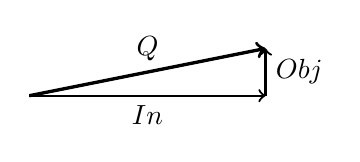
\begin{tikzpicture}
				\pgfmathsetmacro{\phaseLength}{0.6}
				\coordinate (aa) at (0,0);
				\coordinate (bb) at (3,0);
				\coordinate (cc) at (3,\phaseLength);
				% descriptions
				\uncover<2->{\draw[->,thick] (aa) -- (bb) node[midway,below] {$In$};}
				\uncover<3->{\draw[->,thick] (bb) -- (cc) node[midway,right] {$Obj$};}
				\uncover<4->{\draw[->,very thick] (aa) -- (cc) node[midway,above] {$Q$};}
			\end{tikzpicture}
		\end{column}



	\end{columns}
\end{frame}
%%%%%%%%%%%%%%%%%%%%%%%%%%%%%%%%%%%%%%%%%%%%%%%%%%%%%%%%%%%%%%%%%%%%%%%%%%%
\begin{frame}{Transparent Objects in Phase Contrast Microscopy}
	\begin{columns}[T,onlytextwidth]
		\begin{column}{0.6\textwidth}
			\begin{itemize}
				\item<1-> How to covert phase change to amplitude change?
				\item<2-> Apply a filter so that the incident light $In$ is in phase with the specimen effect.
				\item<3-> This can be done at the hardware-level by using a flat sheet of glass.
				\item<4-> The theoretical details can be checked in the course book.
			\end{itemize}
		\end{column}


		\begin{column}{0.4\textwidth}
			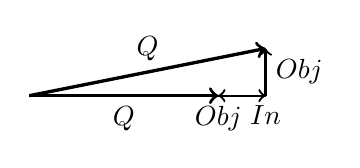
\begin{tikzpicture}
				\pgfmathsetmacro{\phaseLength}{0.6}
				\coordinate (aa) at (0,0);
				\coordinate (bb) at (3,0);
				\coordinate (cc) at (3,\phaseLength);

				\coordinate (cc2) at (3-\phaseLength,0);
				% descriptions
				\uncover<1>{\draw[->,thick] (aa) -- (bb) node[left,below] {$In$};}
				\uncover<1>{\draw[->,thick] (bb) -- (cc) node[midway,right] {$Obj$};}
				\uncover<1>{\draw[->,very thick] (aa) -- (cc) node[midway,above] {$Q$};}
				\uncover<2->{\draw[->,thick] (bb) -- (cc2) node[right,below] {$Obj$};}\pause
				\uncover<2->{\draw[->,very thick] (aa) -- (cc2) node[midway,below] {$Q$};}
			\end{tikzpicture}
		\end{column}



	\end{columns}
\end{frame}

%%%%%%%%%%%%%%%%%%%%%%%%%%%%%%%%%%%%%%%%%%%%%%%%%%%%%%%%%%%%%%%%%%%%%%%%%%%%
\begin{frame}{Phase Contrast Image}
	\begin{figure}
		\begin{subfigure}[t]{0.45\textwidth}
			%\centering
			\includegraphics[width=\textwidth]{images/cells3bfp}
			\caption{A bright field image dominated by almost-transparent objects: adherent ultra-thin CHO cells.}
			\label{fig:mic:cells3bfp}
		\end{subfigure}
		\begin{subfigure}[t]{0.45\textwidth}
			%\centering
			\includegraphics[width=\textwidth]{images/cells3pc}
			\caption{A phase contrast image of the same scene shown in (a).}
			\label{fig:mic:cells3pc}
		\end{subfigure}%
		\caption{Comparison between a phase contrast image and a bright field image.}
		\label{fig:mic:cells3}
	\end{figure}

\end{frame}
%%%%%%%%%%%%%%%%%%%%%%%%%%%%%%%%%%%%%%%%%%%%%%%%%%%%%%%%%%%%%%%%%%%%%%%%%%%
%%%%%%%%%%%%%%%%%%%%%%%%%%%%%%%%%%%%%%%%%%%%%%%%%%%%%%%%%%%%%%%%%%%%%%%%%%%%%%%%%%%%%%%%%%%%%%%%%%%%%%%%%%%%%%

\subsection{Limitation of Light Microscopy}%
\label{sub:limitation_of_light_microscopy}



%%%%%%%%%%%%%%%%%%%%%%%%%%%%%%%%%%%%%%%%%%%%%%%%%%%%%%%%%%%%%%%%%%%%%%%%%%%%%%%%%%%%%%%%%%%%%%%%%%%%%%%%%%%%%%
\begin{frame}{Limitations of Light Microscopy}
	\begin{itemize}
		\item<1-> We learned that it is possible to combine lenses.
		      \begin{itemize}
			      \item<2-> Magnification is the product of the two lens magnifications.
			      \item<3-> Is infinite magnification possible?
		      \end{itemize}
		\item<4-> We have also seen that the image of a \textit{point source} is a \textit{point image}.
		      \begin{itemize}
			      \item<5-> This statement is incorrect.
			      \item<6-> As we will see soon: This implies an upper-limit for the \textit{useful} magnification.
		      \end{itemize}
	\end{itemize}
\end{frame}
%%%%%%%%%%%%%%%%%%%%%%%%%%%%%%%%%%%%%%%%%%%%%%%%%%%%%%%%%%%%%%%%%%%%%%%%%%%
%%%%%%%%%%%%%%%%%%%%%%%%%%%%%%%%%%%%%%%%%%%%%%%%%%%%%%%%%%%%%%%%%%%%%%%%%%%
\begin{frame}{Limitations of Light Microscopy}
	\begin{columns}[c,onlytextwidth]

		\begin{column}{0.6\textwidth}
			\begin{itemize}
				\item<1-> Since light exposes wave-like nature, it suffers from diffraction.
				\item<2-> Due to Diffraction:

				      Image of a point source is not infinitely small (even at best focus).
				      \begin{itemize}
					      \item<3-> It is a pattern called \textbf{Airy pattern}.
					      \item<4-> It is composed of a central spot, known as \textbf{Airy disk}, surrounded by multiple diffraction rings.
					      \item<5-> The radius of Airy disk is:
					            \begin{equation*}\label{eq:mic:airy}
						            \micairy = 0.61\frac{\micwl}{\micna}
					            \end{equation*}
					            $\micwl$ is the wavelength of incident light.
				      \end{itemize}
			\end{itemize}
		\end{column}\uncover<4->{\begin{column}{0.35\textwidth}
				%\begin{figure}
				%\centering
				%		\includegraphics[width=0.5\textwidth]{images/airy-wiki}  
				%		\caption{Image of a point source is Airy pattern in the image plane. Source: Wikipedia.}            
				%\end{figure}
				\centering{}
				\begin{tikzpicture}
					\node[anchor=south west,inner sep=0] at (0,0) {\includegraphics[width=\textwidth]{images/airy-wiki}} {};
					\uncover<5->{\draw[<->,ultra thick] (2.2,2.2) -- (3.1,2.2) node[right,below,yellow] {$\micairy$};}
				\end{tikzpicture}
			\end{column}
		}

	\end{columns}
\end{frame}
%%%%%%%%%%%%%%%%%%%%%%%%%%%%%%%%%%%%%%%%%%%%%%%%%%%%%%%%%%%%%%%%%%%%%%%%%%%
%%%%%%%%%%%%%%%%%%%%%%%%%%%%%%%%%%%%%%%%%%%%%%%%%%%%%%%%%%%%%%%%%%%%%%%%%%%
\begin{frame}[c]{Limitations of Light Microscopy}
	\begin{columns}[c,onlytextwidth]

		\begin{column}{0.6\textwidth}
			\begin{itemize}
				\setlength\itemsep{0.4cm}
				\item<1-> \textbf{\color{faublue}{Intuitively}}:

				      Two objects distinguishable as long as their Airy patterns still distinguishable as two peaks.

				\item<2-> \textbf{\color{faublue}{Resolving power of a microscopic system}}:

				      Minimum distance between two point sources in the object space for which they are still discernible as two points in the image plane.
			\end{itemize}
		\end{column}\begin{column}{0.4\textwidth}
			\uncover<1->{
				\begin{figure}
					%\centering
					\includegraphics[width=0.5\textwidth]{images/rayleigh-wiki-1}
					%\caption{Image of a point source is Airy pattern in the image plane. Source: Wikipedia.}            
					\caption{Separable peaks of Airy patterns}
				\end{figure}
			}

			\uncover<2->{
				\begin{figure}
					%\centering
					\includegraphics[width=0.5\textwidth]{images/rayleigh-wiki-2}
					\caption{Overlapping peaks of Airy patterns}
				\end{figure}
			}
		\end{column}


	\end{columns}
	\begin{flushright}
		\tiny
		Image Source: Wikipedia
	\end{flushright}
\end{frame}
%%%%%%%%%%%%%%%%%%%%%%%%%%%%%%%%%%%%%%%%%%%%%%%%%%%%%%%%%%%%%%%%%%%%%%%%%%%
%%%%%%%%%%%%%%%%%%%%%%%%%%%%%%%%%%%%%%%%%%%%%%%%%%%%%%%%%%%%%%%%%%%%%%%%%%%
\begin{frame}[c]{Limitations of Light Microscopy}
	\begin{columns}[c,onlytextwidth]

		\begin{column}{0.6\textwidth}
			\begin{itemize}
				\item<1-> According to Rayleigh, it is given by the radius of Airy disk:
				      \uncover<2->{
					      \begin{equation*}\label{eq:mic:rayleigh}
						      \micdmin = \micairy = 0.61\frac{\micwl}{\micna}
					      \end{equation*}
				      }
				\item<3-> How to increase resolution?
				      \begin{itemize}
					      \item<4-> Increase numerical aperture.
					            \begin{itemize}
						            \item<5-> $\micna = \micri~ \sin\micla$ is upper-limited by $1$ in air.
						            \item<6-> Use \textbf{oil-immersion} objectives $\micri_{\text{oil}} \approx 1.51$.
					            \end{itemize}
					      \item<7-> Use shorter wavelengths.
				      \end{itemize}
			\end{itemize}
		\end{column}\uncover<1->{\begin{column}{0.35\textwidth}
				\centering{}
				\begin{tikzpicture}
					\node[anchor=south west,inner sep=0] at (0,0) {\includegraphics[width=\textwidth]{images/rayleigh-wiki-2}} {};
					\uncover<2->{\draw[<->,ultra thick] (2.0,1.1) -- (2.6,1.1) node[midway,below,yellow] {$\micdmin$};}
				\end{tikzpicture}
			\end{column}
		}

	\end{columns}
\end{frame}
%%%%%%%%%%%%%%%%%%%%%%%%%%%%%%%%%%%%%%%%%%%%%%%%%%%%%%%%%%%%%%%%%%%%%%%%%%%%%%
%%%%%%%%%%%%%%%%%%%%%%%%%%%%%%%%%%%%%%%%%%%%%%%%%%%%%%%%%%%%%%%%%%%%%%%%%%%
\begin{frame}[c]{Diffraction Limit}
	\begin{columns}[T,onlytextwidth]

		\begin{column}{0.99\textwidth}
			\begin{itemize}
				\setlength\itemsep{0.4cm}
				\item<1-> $\micdmin = \micairy = 0.61\frac{\micwl}{\micna}$

				\item<2-> What is the best theoretically-achievable resolution using visible light?
				      \vspace{0.4cm}

				      \begin{itemize}
					      \setlength\itemsep{0.4cm}
					      \item<3-> Wavelength at the center of visible spectrum $\micwl_{\text{visible}} \approx 550~\micnan$.
					      \item<4-> Setting numerical aperture to the theoretical upper-bound in oil-immersion objectives yields $\micna^{\text{best}} = 1.51$.
					      \item<5-> We obtain a Rayleigh resolution of $\micdmin^{\text{best}} = 222~\micnan \approx 0.2~\micmic$.
					      \item<6-> This value is known as the \textbf{diffraction limit} of visible light.
				      \end{itemize}
			\end{itemize}
		\end{column}

		%\uncover<1->{
		%\begin{column}{0.4\textwidth}			
		%	  \begin{tikzpicture}
		%			\node[anchor=south west,inner sep=0] at (0,0) {\includegraphics[width=\textwidth]{images/rayleigh-wiki-2}} {};
		%			\uncover<1->{\draw[<->,blue,ultra thick] (2.0,1.1) -- (2.6,1.1) node[midway,below] {$\micdmin$};}
		%	  \end{tikzpicture}
		%\end{column}
		%}

	\end{columns}
\end{frame}
%%%%%%%%%%%%%%%%%%%%%%%%%%%%%%%%%%%%%%%%%%%%%%%%%%%%%%%%%%%%%%%%%%%%%%%%%%%
%%%%%%%%%%%%%%%%%%%%%%%%%%%%%%%%%%%%%%%%%%%%%%%%%%%%%%%%%%%%%%%%%%%%%%%%%%%%%%%%%%%%%%%%%%%%%%%%%%%%%%%%%%%%%%


\subsection{Beyond Light Microscopy}%
\label{sub:beyond_light_microscopy}


%%%%%%%%%%%%%%%%%%%%%%%%%%%%%%%%%%%%%%%%%%%%%%%%%%%%%%%%%%%%%%%%%%%%%%%%%%%%%%%%%%%%%%%%%%%%%%%%%%%%%%%%%%%%%%
%%%%%%%%%%%%%%%%%%%%%%%%%%%%%%%%%%%%%%%%%%%%%%%%%%%%%%%%%%%%%%%%%%%%%%%%%%%
\begin{frame}[c]{Beyond Visible Light Microscopy}
	\begin{itemize}
		\setlength\itemsep{0.4cm}
		\item<1-> One obvious way of increasing microscopic resolution is using a wavelength which is shorter than $\micwl_{\text{visible}} \approx 550~\micnan$.
		      \vspace{0.3cm}
		      \begin{itemize}
			      \setlength\itemsep{0.3cm}
			      \item<2-> Ultra-violet (UV) radiation ($300$ -- $100$ $\micnan$).
			      \item<3-> Soft X-ray radiation ($10$ -- $1$ $\micnan$).
			      \item<4-> Hard X-ray radiation (below $1$ $\micnan$).
			      \item<5-> Electron beams (wavelengths below $5$ $\micpic$ are achievable).
		      \end{itemize}
		\item<6-> Each wavelength range allows us to explore a part of the nano-world, but also imposes a new type of challenges for both microscope manufacturers and users.
	\end{itemize}
\end{frame}
%%%%%%%%%%%%%%%%%%%%%%%%%%%%%%%%%%%%%%%%%%%%%%%%%%%%%%%%%%%%%%%%%%%%%%%%%%%
%%%%%%%%%%%%%%%%%%%%%%%%%%%%%%%%%%%%%%%%%%%%%%%%%%%%%%%%%%%%%%%%%%%%%%%%%%%
%%%%%%%%%%%%%%%%%%%%%%%%%%%%%%%%%%%%%%%%%%%%%%%%%%%%%%%%%%%%%%%%%%%%%%%%%%%
\begin{frame}[c]{Challenges with Short Wavelengths}
	\begin{itemize}
		\setlength\itemsep{0.4cm}
		\item<1-> At the UV wavelengths, glass strongly absorbs light radiation.
		\item<2-> At the wavelengths of X-ray radiation, the refractive index of solid substances is very close to the refractive index of air.

		      \begin{itemize}
			      \item<3-> Remember: Light-focusing performed by a visible-light lens is inherently a refraction process.
		      \end{itemize}
		\item<4-> Electron beams need vacuum (no live cell imaging is possible).
		\item<5-> In general, even though very high resolutions are achievable in electron and X-ray microscopy ($0.2$ $\micnan$ in electron microscopy), but:
		      \begin{itemize}
			      \item<5-> They are extremely expensive.
			      \item<6-> Require large hardware.
			      \item<7-> Mostly involve complicated sample preparation.
		      \end{itemize}
	\end{itemize}

\end{frame}
%%%%%%%%%%%%%%%%%%%%%%%%%%%%%%%%%%%%%%%%%%%%%%%%%%%%%%%%%%%%%%%%%%%%%%%%%%%%%%%%%%%%%%%%%%%%%%%%%%%%%%%%%%%%%%

\subsection{Future Trends}%
\label{sub:future_trends}



%%%%%%%%%%%%%%%%%%%%%%%%%%%%%%%%%%%%%%%%%%%%%%%%%%%%%%%%%%%%%%%%%%%%%%%%%%%%%%%%%%%%%%%%%%%%%%%%%%%%%%%%%%%%%%
%%%%%%%%%%%%%%%%%%%%%%%%%%%%%%%%%%%%%%%%%%%%%%%%%%%%%%%%%%%%%%%%%%%%%%%%%%%
%%%%%%%%%%%%%%%%%%%%%%%%%%%%%%%%%%%%%%%%%%%%%%%%%%%%%%%%%%%%%%%%%%%%%%%%%%%%%%%%%%%%%%%%%%%%%%%%%%%%%%%%%%%%%%
\begin{frame}[c]{Future Trends}
	\begin{itemize}
		\setlength\itemsep{0.4cm}
		\item<1-> Light microscopy is very practical compared to electron microscopy, but the latter delivers much higher magnifications.
		\item<2-> Is it possible to break the diffraction limit and thus obtain high magnifications using light microscopy?
		\item<3-> \textbf{Super-resolution} microscopy seems to be the answer (check the course book).
		\item<4-> Stefan Hell was awarded Nobel Prize in Chemistry 2014 for the development of STED (Stimulated Emission Depletion) microscopy: A super-resolution technique which overcomes the diffraction limit of visible light.
	\end{itemize}
\end{frame}
%%%%%%%%%%%%%%%%%%%%%%%%%%%%%%%%%%%%%%%%%%%%%%%%%%%%%%%%%%%%%%%%%%%%%%%%%%%%%%%%%%%%%%%%%%%%%%%%%%%%%%%%%%%%%%




\section{Further Questions?}

\begin{frame}[t]{Further Readings}
	\begin{itemize}
		\item \fullcite{Mualla2018}
	\end{itemize}

\end{frame}




\end{document}
